%%%%%%%%%%%%%%%%%%%%%%%%%%%%%%%%%%%%%%%%%
% Masters/Doctoral Thesis 
% LaTeX Template
% Version 1.41 (9/9/13)
%
% This template has been downloaded from:
% http://www.latextemplates.com
%
% Original authors:
% Steven Gunn 
% http://users.ecs.soton.ac.uk/srg/softwaretools/document/templates/
% and
% Sunil Patel
% http://www.sunilpatel.co.uk/thesis-template/
%
% License:
% CC BY-NC-SA 3.0 (http://creativecommons.org/licenses/by-nc-sa/3.0/)
%
% Note:
% Make sure to edit document variables in the Thesis.cls file
%
%%%%%%%%%%%%%%%%%%%%%%%%%%%%%%%%%%%%%%%%%

%----------------------------------------------------------------------------------------
%	PACKAGES AND OTHER DOCUMENT CONFIGURATIONS
%----------------------------------------------------------------------------------------

\documentclass[12pt, letterpaper, oneside]{Thesis} % Paper size, default font size and one-sided paper
\usepackage{graphicx}
\usepackage[usenames,dvipsnames]{color}
\usepackage{setspace}
\doublespacing
\graphicspath{{Pictures/}} % Specifies the directory where pictures are stored

\usepackage{listings}

\usepackage{color}

\definecolor{mygreen}{rgb}{0,0.6,0}
\definecolor{mygray}{rgb}{0.5,0.5,0.5}
\definecolor{mymauve}{rgb}{0.58,0,0.82}
\definecolor{myred}{rgb}{0.9,0,0.2}
\definecolor{myblue}{rgb}{0,0,1}

\lstset{ %
  backgroundcolor=\color{white},   % choose the background color; you must add \usepackage{color} or \usepackage{xcolor}
  basicstyle=\tiny\ttfamily%\footnotesize,        % the size of the fonts that are used for the code
  breakatwhitespace=false,         % sets if automatic breaks should only happen at whitespace
  breaklines=true,                 % sets automatic line breaking
  captionpos=b,                    % sets the caption-position to bottom
  commentstyle=\color{myblue},    % comment style
  deletekeywords={...},            % if you want to delete keywords from the given language
  escapeinside={\%*}{*)},          % if you want to add LaTeX within your code
  extendedchars=true,              % lets you use non-ASCII characters; for 8-bits encodings only, does not work with UTF-8
  frame=single,                    % adds a frame around the code
  keepspaces=true,                 % keeps spaces in text, useful for keeping indentation of code (possibly needs columns=flexible)
  keywordstyle=\color{blue},       % keyword style
  language=Octave,                 % the language of the code
  morekeywords={*,...},            % if you want to add more keywords to the set
  numbers=left,                    % where to put the line-numbers; possible values are (none, left, right)
  numbersep=5pt,                   % how far the line-numbers are from the code
  numberstyle=\tiny\color{mygray}, % the style that is used for the line-numbers
  rulecolor=\color{black},         % if not set, the frame-color may be changed on line-breaks within not-black text (e.g. comments (green here))
  showspaces=false,                % show spaces everywhere adding particular underscores; it overrides 'showstringspaces'
  showstringspaces=false,          % underline spaces within strings only
  showtabs=false,                  % show tabs within strings adding particular underscores
  stepnumber=2,                    % the step between two line-numbers. If it's 1, each line will be numbered
  stringstyle=\color{mymauve},     % string literal style
  tabsize=2,                       % sets default tabsize to 2 spaces
  title=\lstname                   % show the filename of files included with \lstinputlisting; also try caption instead of title
}



\usepackage{amsmath}

\usepackage{zref-xr}
\zexternaldocument{Chapters/Chapter3_qr_dynamic_model}
\zexternaldocument{Chapters/Chapter4_optimal_control_theory}


\usepackage[square, numbers, comma, sort&compress]{natbib} % Use the natbib reference package - read up on this to edit the reference style; if you want text (e.g. Smith et al., 2012) for the in-text references (instead of numbers), remove 'numbers' 
\hypersetup{urlcolor=blue, colorlinks=true} % Colors hyperlinks in blue - change to black if annoying
\title{\ttitle} % Defines the thesis title - don't touch this

\begin{document}

\frontmatter % Use roman page numbering style (i, ii, iii, iv...) for the pre-content pages

%\setstretch{2} % Line spacing of 1.3

% Define the page headers using the FancyHdr package and set up for one-sided printing
\fancyhead{} % Clears all page headers and footers
\rhead{\thepage} % Sets the right side header to show the page number
\lhead{} % Clears the left side page header

\pagestyle{fancy} % Finally, use the "fancy" page style to implement the FancyHdr headers

\newcommand{\HRule}{\rule{\linewidth}{0.5mm}} % New command to make the lines in the title page
\newcommand{\p}{\partial}
\newcommand{\spa}{\text{ }}
\newcommand{\cc}{\mathfrak{C}} % note this must appear in math mode
% PDF meta-data
\hypersetup{pdftitle={\ttitle}}
\hypersetup{pdfsubject=\subjectname}
\hypersetup{pdfauthor=\authornames}
\hypersetup{pdfkeywords=\keywordnames}

%----------------------------------------------------------------------------------------
%	TITLE PAGE
%----------------------------------------------------------------------------------------

\begin{titlepage}
\begin{center}

QUADROTOR FLIGHT PATH ENERGY OPTIMIZATION
\vspace{15 mm}

By Edward Kemper

A Thesis

Submitted in Partial Fulfillment

of the requirements for the degree of 

Masters of Science

in Electrical Engineering
\vspace{15 mm}

Northern Arizona University

April 2014
\vspace{20 mm}

Approved:

Dr. Niranjan Venkatraman, Ph.D.,Chair

Dr. Sheryl Howard, Ph.D.

Dr. Allison Kipple, Ph.D.




\vfill
\end{center}

\end{titlepage}

%----------------------------------------------------------------------------------------
%	DECLARATION PAGE
%	Your institution may give you a different text to place here
%----------------------------------------------------------------------------------------
%
%\Declaration{
%
%\addtocontents{toc}{\vspace{1em}} % Add a gap in the Contents, for aesthetics
%
%I, \authornames, declare that this thesis titled, '\ttitle' and the work presented in it are my own. I confirm that:
%
%\begin{itemize} 
%\item[\tiny{$\blacksquare$}] This work was done wholly or mainly while in candidature for a research degree at this University.
%\item[\tiny{$\blacksquare$}] Where any part of this thesis has previously been submitted for a degree or any other qualification at this University or any other institution, this has been clearly stated.
%\item[\tiny{$\blacksquare$}] Where I have consulted the published work of others, this is always clearly attributed.
%\item[\tiny{$\blacksquare$}] Where I have quoted from the work of others, the source is always given. With the exception of such quotations, this thesis is entirely my own work.
%\item[\tiny{$\blacksquare$}] I have acknowledged all main sources of help.
%\item[\tiny{$\blacksquare$}] Where the thesis is based on work done by myself jointly with others, I have made clear exactly what was done by others and what I have contributed myself.\\
%\end{itemize}
% 
%Signed:\\
%\rule[1em]{25em}{0.5pt} % This prints a line for the signature
% 
%Date:\\
%\rule[1em]{25em}{0.5pt} % This prints a line to write the date
%}

%\clearpage % Start a new page

%----------------------------------------------------------------------------------------
%	QUOTATION PAGE
%----------------------------------------------------------------------------------------

%\pagestyle{empty} % No headers or footers for the following pages

%\null\vfill % Add some space to move the quote down the page a bit

%\textit{``Thanks to my solid academic training, today I can write hundreds of words on virtually any topic without possessing a shred of information, which is how I got a good job in journalism."}

%\begin{flushright}
%Dave Barry
%\end{flushright}

%\vfill\vfill\vfill\vfill\vfill\vfill\null % Add some space at the bottom to position the quote just right

%\clearpage % Start a new page

%----------------------------------------------------------------------------------------
%	ABSTRACT PAGE
%----------------------------------------------------------------------------------------

\addtotoc{Abstract} % Add the "Abstract" page entry to the Contents

\abstract{\addtocontents{toc}{\vspace{1em}} % Add a gap in the Contents, for aesthetics

Quad-Rotor UAVs have been a popular area of research and development in the last decade, especially with the advent of affordable microcontrollers like the MSP 430 and the Raspberry Pi. Path-Energy Optimization is an area that is well developed for linear systems. In this thesis, this idea of path-energy optimization is extended to the nonlinear model of the Quad-rotor UAV. The classical optimization techniques is adapted to the nonlinear model that is derived for the problem at hand, coming up with a set of partial differential equations and boundary value conditions to solve these equations. Then, different techniques to implement energy optimization algorithms are tested using simulations in Python. First, a purely nonlinear approach is used. This method is shown to be computationally intensive, with no practical solution available in a reasonable amount of time. Second, heuristic techniques to minimize the energy of the flight path is tested, using Ziegler-Nichols' PID tuning technique. Finally, a brute force lookup table based PID controller is used. Simulation results of the heuristic method show both reliable control of the system and path-energy optimization are achieved in a reasonable amount of time.

%In this thesis we develop and compare two methods for the energy optimization of a quad rotor UAV flight path between two known points. First, we use classical optimal control techniques and find an approximate solution to the resulting boundary value problem. This method is shown to be too computationally intensive to %provide a solution in a reasonable amount of time. The second method that is developed is a heuristic technique which minimizes the energy of the flight path through optimal PID controller tuning. Simulation results of the heuristic method show that both reliable control of the system and energy minimization are achieved. %{\color{red}WHAT SPECIFIC CHANGES / ADDITIONS ARE NEEDED HERE}
%}

\clearpage % Start a new page

%----------------------------------------------------------------------------------------
%	ACKNOWLEDGEMENTS
%----------------------------------------------------------------------------------------

%\setstretch{1.3} % Reset the line-spacing to 1.3 for body text (if it has changed)

\acknowledgements{\addtocontents{toc}{\vspace{1em}} % Add a gap in the Contents, for aesthetics

There are a great many people who need to be recognized for their contribution to the success of my academic endeavors. Thank you to my parents for their continued financial and moral support. Thank you to Terry Halmo, Dr. Monty Mola, Dr. Wes Bliven, Dr. Robert Zoellner, and the rest of the Physics and Chemistry Faculty at Humboldt State for their work in mentoring and teaching. Thank you to Dr. Allison Kipple, Dr. Sheryl Howard, Dr. Paul Flikkema, Dr. Phillip Mlsna, and the rest of the Engineering Faculty at NAU. Thank you to Emily, my partner, for taking in stride the rich insanity of math and code that sometimes dominates my being. Finally thank you to Dr. Niranjan Venkatraman for his continuous, enthusiastic involvement in the development of this thesis. 
}
\clearpage % Start a new page

%----------------------------------------------------------------------------------------
%	LIST OF CONTENTS/FIGURES/TABLES PAGES
%----------------------------------------------------------------------------------------

\pagestyle{fancy} % The page style headers have been "empty" all this time, now use the "fancy" headers as defined before to bring them back

\lhead{Contents} % Set the left side page header to "Contents"
\tableofcontents % Write out the Table of Contents

\lhead{List of Figures} % Set the left side page header to "List of Figures"
\listoffigures % Write out the List of Figures

%\lhead{\emph{List of Tables}} % Set the left side page header to "List of Tables"
%\listoftables % Write out the List of Tables

%----------------------------------------------------------------------------------------
%	ABBREVIATIONS
%----------------------------------------------------------------------------------------

%\clearpage % Start a new page

%\setstretch{1.5} % Set the line spacing to 1.5, this makes the following tables easier to read

%\lhead{\emph{Abbreviations}} % Set the left side page header to "Abbreviations"
%\listofsymbols{ll} % Include a list of Abbreviations (a table of two columns)
%{
%\textbf{LAH} & \textbf{L}ist \textbf{A}bbreviations \textbf{H}ere \\
%\textbf{Acronym} & \textbf{W}hat (it) \textbf{S}tands \textbf{F}or \\
%}

%----------------------------------------------------------------------------------------
%	PHYSICAL CONSTANTS/OTHER DEFINITIONS
%----------------------------------------------------------------------------------------

%\clearpage % Start a new page

%\lhead{\emph{Physical Constants}} % Set the left side page header to "Physical Constants"

%\listofconstants{lrcl} % Include a list of Physical Constants (a four column table)
%{
%Speed of Light & $c$ & $=$ & $2.997\ 924\ 58\times10^{8}\ \mbox{ms}^{-\mbox{s}}$ (exact)\\



% Constant Name & Symbol & = & Constant Value (with units) \\
%}

%----------------------------------------------------------------------------------------
%	SYMBOLS
%----------------------------------------------------------------------------------------

%\clearpage % Start a new page
%
%\lhead{\emph{Symbols}} % Set the left side page header to "Symbols"
%
%\listofnomenclature{lll} % Include a list of Symbols (a three column table)
%{
%$a$ & distance & m \\
%$P$ & power & W (Js$^{-1}$) \\
% Symbol & Name & Unit \\
%
%& & \\ % Gap to separate the Roman symbols from the Greek
%
%$\omega$ & angular frequency & rads$^{-1}$ \\
% Symbol & Name & Unit \\
%}

%----------------------------------------------------------------------------------------
%	DEDICATION
%----------------------------------------------------------------------------------------

%\setstretch{1.3} % Return the line spacing back to 1.3

\pagestyle{empty} % Page style needs to be empty for this page

\dedicatory{For my Parents Jack and Carol\ldots} % Dedication text

\addtocontents{toc}{\vspace{2em}} % Add a gap in the Contents, for aesthetics

%----------------------------------------------------------------------------------------
%	THESIS CONTENT - CHAPTERS
%----------------------------------------------------------------------------------------

\mainmatter % Begin numeric (1,2,3...) page numbering

\pagestyle{fancy} % Return the page headers back to the "fancy" style

% Include the chapters of the thesis as separate files from the Chapters folder
% Uncomment the lines as you write the chapters

% Chapter 1

\chapter{Introduction} % Main chapter title

\label{Introduction} % For referencing the chapter elsewhere, use \ref{Chapter1}

%\lhead{Chapter 1. \emph{Introduction}} % This is for the header on each page - perhaps a shortened title

%-------------------------------------------------------------- --------------------------

The technology surrounding Unmanned Aerial Vehicles (UAVs), and in particular quad-rotor devices, has seen tremendous development in recent years. Likewise, the creative application of this technology has expanded into many contexts. Like many new technologies, the early development of UAVs was mostly in a military context. This is not the case any more. The private sector has taken a huge interest in this technology. There is a wide range of companies contributing to the development of UAV technology from open-source projects like DIY Drones \cite{diydrones:2014:Online} to start-up firms backed by Google, such as Airware \cite{Airware:2014:Online}.  The Federal Aviation Administration in the USA has plans to produce concrete policy regarding the regulation of commercial applications of UAVs by 2015 \cite{faa:2014:Online}. This will sow the seeds for the rapid growth of a multi-billion dollar industry. There are many applications for this technology which have the potential to save lives and collect scientific data that could inform state and federal legislation. Certainly, the range of potential applications will be further diversified as the technology sees more development.

Unmanned Ariel Vehicles are also called by various other names: remotely piloted vehicles (RPVs), remote controlled drones, robot planes, and pilot-less aircraft. Such vehicles are defined as powered, aerial vehicles that do not carry a human operator and can use aerodynamics forces to provide vehicle lift. They can fly autonomously or be piloted remotely, can be expendable or recoverable, and can carry a lethal or nonlethal payload \cite{bone2004unmanned}.


\section{Motivation}

With many private organizations making use of UAVs for a variety of applications, one pervasive engineering problem that still exists in general is that of managing the energy usage. Quad-rotors specifically are plagued by very high energy demand. There are two different kinds of UAVs: fixed wing, which have the ability to soar or glide, and multi-rotor systems, which are entirely thrust-driven. It is the natural instability of multi-rotor UAVs which make them extremely maneuverable, but this comes at the cost of high energy expenditure. This provides the motivation for this thesis - to develop an optimal control technique that optimizes the path-energy of a quad-copter UAV.


\section{Prior Work}

There have been work published on the energy optimization and trajectory planning of fixed wing UAVs. Given the ability to soar and utilize thermal gradients in the atmosphere, it is suggested that fixed wing UAVs have the potential to stay aloft almost permanently \cite{langelaan2007long}, \cite{klesh2009solar}, and \cite{lawrance2009guidance}.  This makes fixed wing UAVs ideal for applications like aerial surveys or surveillance missions. These aircrafts have the major disadvantage that they are dependent upon some kind of launching mechanism, or a runway, for takeoff and landing.

In contrast, rotary wing UAVs have a higher degree of mechanical complexity. These UAVs can take off and land vertically and have the capacity to hover. This makes rotary wing UAVs, such as the quad-copter, more suitable for short range search and rescue missions, facility inspections, and single-target tracking. Since fixed wing and multi-rotor UAVs are fundamentally different in their physical operation, procedures for managing their respective energy usage are also necessarily unique.

In academic contexts, many advances in UAV and specifically quad-rotor research have provided the seeds for growth for this industry. The problem of basic stability and position control is solved in \cite{erginer2007modeling}, \cite{bouabdallah2004pid}, and \cite{Luukkonen}.


The background material for understanding the dynamical model of the quad-rotor as given by the Euler-Lagrange formulation is explained in \cite{marion1995classical} and  \cite{cornelius1970variational}. These references provide detailed derivations and discussions of the Euler-Lagrange equations of motion as well as related topics like Hamiltonian mechanics and the calculus of variations. Also, \cite{cornelius1970variational} provides an in-depth review of the historical context surrounding the development of classical mechanics. The derivation of the quad-rotor dynamical model as well as attitude and position control via PD or PID controllers is discussed in \cite{erginer2007modeling}, \cite{bouabdallah2004pid}, and  \cite{Luukkonen}. These papers provide derivations of both the Euler-Lagrange and Newtonian formulations for the quad-rotor.

Optimal control was born in 1697, when Johann Bernoulli published his solution to the Brachystochrone problem in \cite{JBernoulli} . With the work of Bernoulli, Newton, Leibniz, l'Hopital, and Tschirnhaus, the field of optimal control was clearly defined. This was followed by the works of Euler, Lagrange, and Legendre which led to the fundamental optimization equations, Euler's equation \cite{LEuler}, the Euler-Lagrange formulation, and Legendre's necessary condition for a minimum. W. R. Hamilton then came up with an equivalent to the Euler-Lagrange equation that could be used in deriving control equations. This was known as the control Hamiltonian form of the Euler-Lagrange equations. The next development was from Weierstass, who came up with the fundamental path optimization problem in optimal control theory in the late 19th century. This was followed by the fundamental minimization principle by Pontryagin that allows for solving most optimization problems \cite{Pontry}. Several books on optimal control (\cite{lewis2012optimal} , \cite{BrysonHo69}, \cite{locatelli2001optimal}, \cite{athans2006optimal}) were referenced for the derivations used in this thesis. In order to test the nonlinear optimization, numerical algorithms for the shooting method (\cite{richard1988douglas}, \cite{rao2009engineering}, \cite{keller1992numerical}) and the finite difference method (\cite{rao2009engineering}, \cite{keller1992numerical}) were used.

The Proportional-Integral-Derivative (PID) controller is a control loop feedback mechanism widely used to drive a system to a desired set point. The mechanism uses an error value as the input to the controller. PID controllers are common in industrial applications \cite{o2006reducing}. In the absence of the knowledge of an underlying process, the PID is considered the best method of control. It must be noted that PID controllers do not necessarily result in optimal control of the system. However, it is possible to achieve a desired system response by adjusting the mathematical parameters of the control expressions. This process is called ``tuning''. The tuning must satisfy many criteria within the limitations of PID control and the system itself. There are various tuning techniques \cite{bequette2003process}. For instance, there are the Ziegler-Nichols, manual tuning, and software tuning methods which can be applied to other control problems \cite{AngChong}, \cite{Bennett}.


\section{Organization of the Thesis}

The objective of this thesis is to develop a path-energy optimization technique that can operate on a near real-time schedule. Two different methods are discussed. We compare a classical optimal control technique with a simpler heuristic approach involving PID controller tuning. The organization of the chapters is as follows.

In Chapter 2, we present a detailed problem statement where the goal of the research project is defined. Chapter 3 uses the Euler-Lagrange equations of motion to derive a nonlinear dynamical model for the quad-rotor UAV. This mathematical model is the basis of the development of the control and energy optimization algorithms. In chapter 4, we define the various optimality conditions. Then we and formulate a generalized, classical optimal control scheme. Then we solve the boundary value problem generated by two methods and discuss their pros and cons. In Chapter 5, the classical optimal control scheme developed in the previous chapter is applied to the quad-rotor UAV. The resulting boundary value problem and its solution method is discussed. Chapter 6 deals with the PID/PD control technique. The control expressions are derived, and the method is tested. Results from these tests are discussed. Chapter 7 outlines a heuristic approach to the path-energy optimization problem and presents the simulation results of the control algorithm developed. Chapter 8 summarizes the results and proposes avenues for continued research.













% Chapter Template

\chapter{Problem Statement} % Main chapter title

\label{Chapter2} % Change X to a consecutive number; for referencing this chapter elsewhere, use \ref{ChapterX}

\lhead{Chapter 2. \emph{Problem Statement}} % Change X to a consecutive number; this is for the header on each page - perhaps a shortened title



We wish to find a set of control expressions for a quad-rotor UAV which minimizes the energy expended in flying between two known 3D points. In order to maintain focus on a tractable problem, some mathematical assumptions are made about the scenario. First, we assume that the flight path that will be optimized is free of obstacles. Second, we assume only modeled environmental variables. We use a mathematical model of the system derived from a Euler-Lagrange formulation as in \cite{Luukkonen} and \cite{bouabdallah2004pid}. 

In the classical optimal control approach,\cite{BrysonHo69} \cite{kirk70} {\color{red}WHY IS THIS REFERENCE BROKEN???} \cite{lewis2012optimal}, the control of the system and the optimization are represented in a single mathematical formulation. Solving the optimal control problem is achieved by solving a boundary value problem. For a highly non-linear system such as a quad-rotor, this becomes extremely involved. The classical optimal control approach is shown to be too computationally intensive for a real-time implementation because the result is a monstrous two point boundary value problem. Solving the theoretical optimal control problem would likely produce accurate results, but only after an inordinate lapse of time for computation. Also, the convergence of the solution is shown to be intermittent. 

 For our heuristic approach, full control of the UAV is attained by using PD attitude controllers in conjunction with PID controllers for position. This provides a platform for simulating the UAV as it flies from a known initial position to a desired set point location. The optimization procedure evaluates the results of these simulations for optimality as a function of the PID gains used in the position control expressions.   

It is pertinent to define what is meant by near real-time in our somewhat sterile mathematical context. We assume that the set of initial and final locations of the quad-rotor are defined by a user on a human time scale. Imagine a graphical user interface in which the desired location of the UAV is programmed. The quad-rotor then physically traverses the optimal path without more than a second or two of computation before the flight begins. For an autonomous UAV, the on board computational resources define an upper limit to the computational complexity of the control algorithm. It is our aim to design an energy optimized control scheme which meets these constraints. 


% Chapter Template

\chapter{Quadrotor Dynamic Model} % Main chapter title

\label{Chapter2} % Change X to a consecutive number; for referencing this chapter elsewhere, use \ref{ChapterX}

\lhead{Chapter 2. \emph{Quadrotor Dynamic Model}} % Change X to a consecutive number; this is for the header on each page - perhaps a shortened title

%----------------------------------------------------------------------------------------
%	SECTION 1
%----------------------------------------------------------------------------------------

In this chapter, a mathematical model of the quad-rotor is derived. This model will be used as the basis for the optimization techniques outlined in subsequent chapters.

\section{Description of a quad-rotor}

In general, a quad-rotor is physically composed of a simple frame supporting four brush-less motors. Thrust is provided by propellers attached to these motors. The speeds of the rotors are governed by a control algorithm which is implemented on some form of on board processor.

 The stabilization and control of a quad-rotor is accomplished by varying the speeds of the motors. The thrust the in vertical direction is controlled by varying all four motor speeds uniformly. In the quad-rotor frame of reference, the direction of the thrusts from the motors is fixed. This means that in order to produce lateral motion, the UAV must tilt such that a component of the total thrust vector points in the desired direction of motion. The pitch and roll angular positions are controlled by driving motors on opposite sides of the frame at different speeds. This produces torque about the center of mass of the quad-rotor. Given non-zero pitch, roll, and total thrust, the UAV experiences horizontal linear acceleration. The yaw angular position is controlled by driving pairs of opposite motors at the different speeds. This produces a torque about the yaw axis but not about the pitch or roll axes. Also, the two opposite pairs of motors must spin in opposite directions so that when hovering, the net torque about the yaw axis is zero. The details of this description are represented mathematically in the next section.



\section{Euler-Lagrange Formulation}

In order to implement a control algorithm, we must understand the mathematical relationships between the control input and the resulting dynamics of the system. Using the Euler-Lagrange formulation from classical mechanics, we can obtain a nonlinear, deterministic dynamical model. General derivation of the Euler Lagrange differential equations of motion can be found in \cite{marion1995classical} and  \cite{cornelius1970variational}.

 The linear and angular coordinates are defined as in Figure \ref{fig:quad-rotor coordinate system}.

\begin{figure}[htbp]
	\centering
		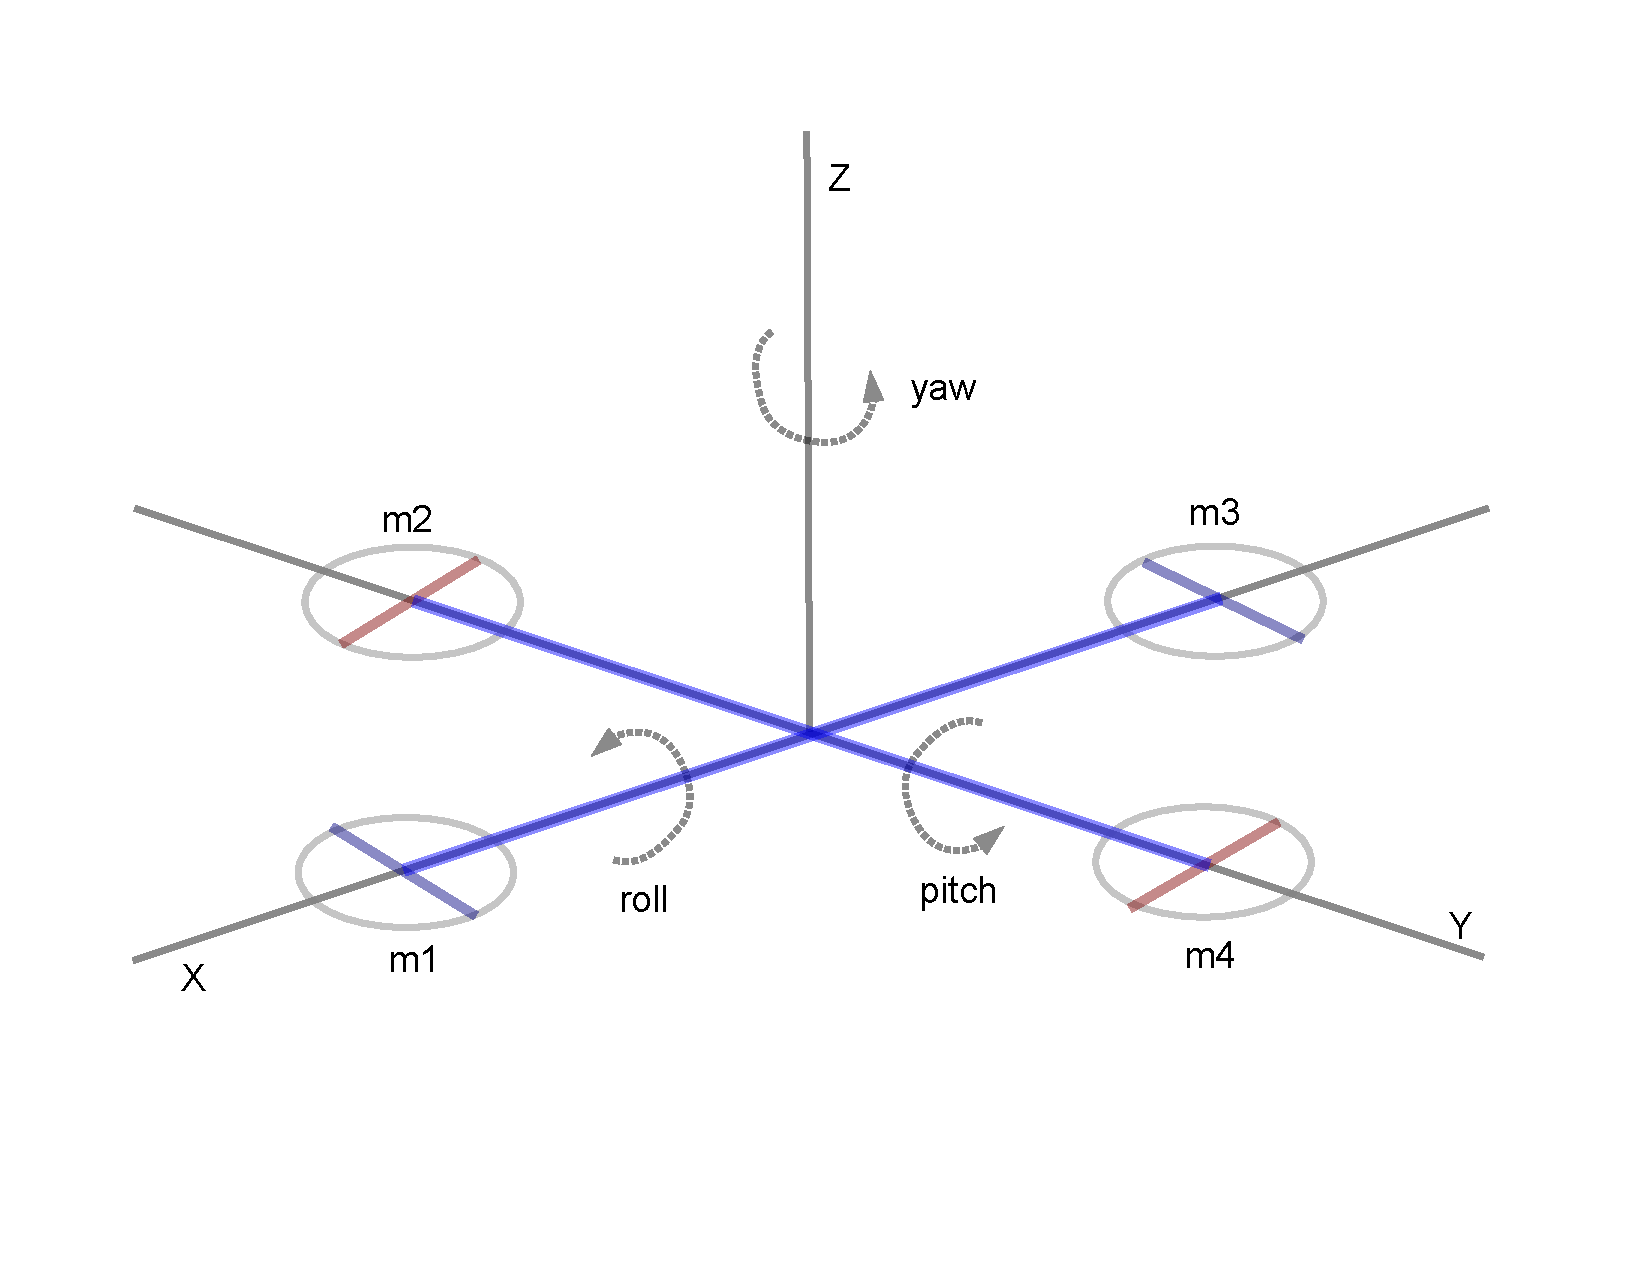
\includegraphics[width=\textwidth]{Figures/coords.pdf}
		\rule{35em}{0.5pt}
	\caption[quad-rotor coordinate system]{quad-rotor coordinate system}
	\label{fig:quad-rotor coordinate system}
\end{figure}


\indent $ \psi $ is the yaw angle around the z-axis\\
\indent $ \theta $ is the pitch angle around the y-axis\\
\indent $ \phi $ is the roll angle around the x-axis\\

$\boldsymbol \xi = \left[ \begin{array}{c}
x\\y\\z\\
\end{array} \right] $, $\boldsymbol \eta =  \left[ \begin{array}{c}
\phi\\\theta\\\psi\\
\end{array} \right] $, $\boldsymbol q = \left[ \begin{array}{c}
\xi\\\eta\\
\end{array} \right]$\\

The coordinates  $ q_i=\{x,y,z,\psi ,\theta ,\phi \} $  are in reference to a ground based inertial coordinate system. The system states and control inputs must be mapped from the quad-rotor frame of reference to the inertial frame in order to express the dynamics of the system. The matrix below represents an arbitrary rotation transformation from the body frame to the inertial frame is:

\begin{equation}
\boldsymbol R = \left[ \begin{array}{ccc}
c(\psi) c(\theta) & c(\psi) s(\theta) s(\phi) - s(\psi) c(\phi) & c(\psi) s(\theta) c(\phi) + s(\psi) s(\phi)\\
s(\psi) c(\theta) & s(\psi) s(\theta) s(\phi) + c(\psi) c(\phi) & s(\psi) s(\theta) c(\phi) - c(\psi) s(\phi)\\
-s(\theta) & c(\theta) s(\phi) & c(\theta) c(\phi)\\
\end{array} \right]\\
\end{equation}

For simplicity, cos is denoted by 'c' and sin is denoted by 's' in the above expression. 



\noindent 
The mass of the quad-rotor is $m$. Each of the moments of inertia  $ i_{xx} $  and $ i_{yy} $
are assumed to be composed of a rod of length $ L $   which accounts for half of the mass of the quad-rotor. Assume the mass
is evenly distributed along the two perpendicular rods. Let  \(\beta  =\text{  }\frac{1}{12}m l^2 \). The inertia matrix for the quad-rotor is then: \\

\begin{equation}
I = \left(
\begin{array}{ccc}
 \frac{1}{12}\left(\frac{m}{2}\right)l^2 & 0 & 0 \\
 0 & \frac{1}{12}\left(\frac{m}{2}\right)l^2 & 0 \\
 0 & 0 & \frac{1}{12}m l^2 \\
\end{array}
\right) = \left(
\begin{array}{ccc}
 \frac{\beta }{2} & 0 & 0 \\
 0 & \frac{\beta }{2} & 0 \\
 0 & 0 & \beta  \\
\end{array}
\right).
\end{equation}

\noindent In the inertial frame, the kinetic and potential energy of the system are given by

%translational kinetic energy
\begin{equation}
    T_{\text{trans}}=\frac{1}{2}m\dot{\xi }^T\dot{\xi }
\end{equation}


%rotational kinetic energy
\begin{equation}
    T_{\text{rot}}= \frac{1}{2}\dot{\eta }^T J \dot{\eta } 
\end{equation}


% system potential energy
\begin{equation}
    U = m g z.
\end{equation}


The Lagrangian is formed as the difference between kinetic and potential energy.

\begin{equation}
    L = \frac{1}{2}m\dot{\xi }^T\dot{\xi }+\frac{1}{2}\dot{\eta }^T   J   \dot{\eta }\text{  }- m g z
\end{equation}

Where $J$ is the Jacobian for transforming the angular velocities from the quad-rotor body frame to the inertial frame.

\begin{equation}
    J = W_{\eta}^T I W_{\eta} 
\end{equation}

\begin{equation}
\boldsymbol W_{\eta} = \left[ \begin{array}{ccc}

1 & 0 & -sin(\theta)\\ 0 & cos(\phi) & cos(\theta) sin(\phi)\\ 0 & -sin(\phi) & cos(\theta) cos(\phi)\\

\end{array} \right]
\end{equation}



\noindent The matrix $\boldsymbol W_{\eta}$ is ...{\color{red} need a good explanation of the W matrix, there is some subtle math here that needs to be clarified}




\begin{equation}
J= \left(
\begin{array}{ccc}
 \frac{\beta }{2}    & 0                                                                    & -\frac{\beta }{2}s(\theta) \\
 0                   & \frac{\beta}{2} c(\phi)^2 + \beta s(\phi)^2                       & \frac{- \beta}{2} c(\phi) \text{ } s(\phi) \text{ } c(\theta)  \\
 -\beta s(\theta)   & \frac{- \beta}{2} c(\phi) \text{ } s(\phi) \text{ } c(\theta)    & \frac{\beta }{2}s(\theta)^2 + \frac{\beta }{2} s(\phi)^2  c(\theta)^2 + \beta  c(\phi)^2  c(\theta)^2  \\
\end{array}
\right)
\end{equation}




\noindent The dynamics of the system are represented by the Euler - Lagrange differential equations of motion.

\begin{equation}
    \frac{d}{\text{dt}} \left( \frac{\delta  L} {\delta \dot{q}}\right) - \frac{\delta  L}{\delta q}=F 
\end{equation}


$ q = \{x,y,z,\psi ,\theta ,\phi \} = \{ \xi , \eta \}  $.


\noindent  $ f $ is the generalized force vector representing the linear external force acting on the system. 
$\tau_b $ are the torques acting on the system due to the rotors.

\begin{equation}
    \left( \begin{array}{c} f \\ \tau \\ \end{array} \right) = \frac{d}{\text{dt}} \left( \frac{\delta  L} {\delta \dot{q}}\right) - \frac{\delta  L}{\delta q}
\end{equation}

General derivations of the Euler-Lagrange equations of motion can be found in \cite{marion1995classical} and  \cite{cornelius1970variational}. 





\noindent The linear components of the generalized forces produce the following equations.

\begin{equation}
    f =  R  T_B = m \ddot{ \xi} -  G
\end{equation}


\begin{equation}
    m\left(\begin{array}{c}
      \ddot{x}\\
      \ddot{y}\\
      \ddot{z}\\
    \end{array}\right)
    - \left( \begin{array}{c}
        0\\
        0\\
        -m g  
      \end{array} \right)
      =u
     \left(
    \begin{array}{c}
     \cos{\psi}\sin{\theta}\cos{\phi} + \sin{\psi}\sin{\phi} \\
     \sin{\psi}\sin{\theta}\cos{\phi} - \cos{\psi}\sin{\phi} \\
     \cos{\theta} \cos{\phi} \\
    \end{array}
    \right)
\end{equation}


\noindent The angular components are expressed as

\begin{equation}
    \tau = \tau_b =\frac{d}{dt} \left( \frac{\partial  L} {\partial \dot{\eta}}\right) - \frac{\partial  L}{\partial \eta}
\end{equation}

\begin{equation}
    \tau_b =\frac{d}{dt} ( J \dot{\eta} ) - \frac{1}{2} \frac{\partial}{\partial \eta} ( \dot{\eta}^T J \dot{\eta}  ) 
\end{equation}

\begin{equation}
    \tau_b =J \ddot{\eta} + \frac{d}{dt}(J) \dot{\eta} - \frac{1}{2} \frac{\partial}{\partial \eta} ( \dot{\eta}^T J \dot{\eta}  ) 
\end{equation}

\begin{equation}
    \tau_b =  J \ddot{\eta} + \cc(\eta,\dot{\eta}) \dot{\eta} 
\end{equation}

\begin{equation}
    \label{eq:angularacc}
    \ddot{\eta} = J^{-1} \big( \tau_b - \cc(\eta,\dot{\eta}) \dot{\eta} \big) 
\end{equation}


The Coriolis matrix is defined as follows. {\color{red} NEED A REFEREED DOCUMENT WITH THE DERIVATION}



\begin{equation}
    \cc(\eta,\dot{\eta}) = 
    \left(
        \begin{array}{c c c}
            \cc_{(11)} & \cc_{(12)} & \cc_{(13)} \\
            \cc_{(21)} & \cc_{(22)} & \cc_{(23)} \\
            \cc_{(31)} & \cc_{(32)} & \cc_{(33)} \\
        \end{array}
    \right)
\end{equation}




$\cc_{(11)} = 0$

$\cc_{(12)}  = (I_{yy}-I_{zz})  ( \dot{\theta} C_{\phi} S_{\phi} +  \dot{\psi} C_{\theta} S_{\phi}^2 )  + (I_{zz}-I_{yy})  \dot{\psi} C_{\phi}^2 C_{\theta} - I_{xx}  \dot{\psi} C_{\theta}$


$\cc_{(13)} = (I_{zz}-I_{yy})    \dot{\psi}   C_{\phi}   S_{\phi}  C_{\theta}^2$


$\cc_{(21)} = (I_{zz}-I_{yy})   ( \dot{\theta} C_{\phi} S_{\phi} +  \dot{\psi} S_{\phi} C_{\theta} ) + (I_{yy}-I_{zz})    \dot{\psi}   C_{\phi}^2  C_{\theta} + I_{xx}    \dot{\psi}   C_{\theta}$


$\cc_{(22)}  = (I_{zz}-I_{yy}) \dot{\phi} C_{\phi} S_{\phi}$


$\cc_{(23)}  = -I_{xx}  \dot{\psi} S_{\theta} C_{\theta} + I_{yy}  \dot{\psi} S_{\phi}^2 S_{\theta} C_{\theta} + I_{zz} \dot{\psi} C_{\phi}^2 S_{\theta} C_{\theta}$


$\cc_{(31)} = (I_{yy}-I_{zz}) \dot{\psi} C_{\theta}^2 S_{\phi} C_{\phi} - I_{xx} \dot{\theta} C_{\theta}$


$\cc_{(32)}  = (I_{zz}-I_{yy}) ( \dot{\theta} C_{\phi} S_{\phi} S_{\theta} + \dot{\phi} S_{\phi}^2 C_{\theta} ) + (I_{yy}-I_{zz}) \dot{\phi} C_{\phi}^2 C_{\theta} + I_{xx}  \dot{\psi} S_{\theta} C_{\theta} - I_{yy}  \dot{\psi} S_{\phi}^2 S_{\theta} C_{\theta} - I_{zz}  \dot{\psi} C_{\phi}^2 S_{\theta} C_{\theta}$


$\cc_{(33)} = (I_{yy}-I_{zz})   \dot{\phi}  C_{\phi} S_{\phi} C_{\theta}^2 - I_{yy}   \dot{\theta} S_{\phi}^2 C_{\theta} S_{\theta} - I_{zz} \dot{\theta} C_{\phi}^2 C_{\theta} S_{\theta} + I_{xx} \dot{\theta} C_{\theta} S_{\theta}$\\



%-------------------------------------------------------------------------
 
In general, the Coriolis term is a mathematical result of the rotational motion of one coordinate system with respect to another. Since we are considering arbitrary three dimensional motion, there are three orthogonal axes of rotation and the resulting matrix is quite complicated. According to the expression for the angular acceleration (equation \eqref{eq:angularacc}), the physical units of the Coriolis term must be torque to maintain algebraic continuity. It is important to keep in mind that the Coriolis term does not represent a real force or torque acting on the system. It is only an artifact which is needed to account for the relative rotation of one coordinate frame with respect to another.   




\section{Motor Speeds, Thrust and Torque}

\indent The rotor angular velocities are related to the forces they produce by $f_i = s \omega^2_i$ where s is the constant of proportionality.
The torques due to the rotors about the rotors' axes of rotation are given by $\tau_{M_i} = b \omega^2_i + I_M \dot{\omega}_i$. The parameter b is a drag coefficient. Note the effect of $\dot{\omega}_i$ is considered to be negligible because the rotational inertia of the rotor itself is negligible.

In the quad-rotor frame of reference, the motors produce torques on the system.

\begin{equation}
    \label{taub}
    \boldsymbol \tau_B = \left[ \begin{array}{c} \tau_{\phi}\\\tau_{\theta}\\\tau_{\psi}\\ \end{array} \right] = \left[ \begin{array}{c} l s (-\omega_2^2 + \omega_4^2)\\l s (-\omega_1^2 + \omega_3^2)\\ \displaystyle \sum \limits_{i=1}^4 b \omega^2\\\end{array} \right]
\end{equation}

The combined thrust of the rotors in the direction of the quad-rotor frame $z$ axis is\\

$\boldsymbol T_B = \left[ \begin{array}{c} 0\\0\\T\\ \end{array} \right]$ where,\\

\begin{equation}
    \label{totalThrust}
    T =  \displaystyle \sum \limits_{i=1}^4 f_i
\end{equation}



\section {A Complete Model}


A complete mathematical representation of the quad-rotor is as follows.\\ 

\begin{equation}
    \left(
        \begin{array}{c}
           \ddot{x}\\
           \ddot{y}\\
           \ddot{z}\\
        \end{array}
    \right)
    = \left(
       \begin{array}{c}
        0\\
        0\\
        g  
      \end{array}
    \right)
    +\frac{T}{m}
     \left(
        \begin{array}{c}
             C_{\psi}S_{\theta}C_{\phi} + S_{\psi}S_{\phi} \\
             S_{\psi}S_{\theta}C_{\phi} - C_{\psi}S_{\phi} \\
             C_{\theta} C_{\phi} \\
        \end{array}
    \right)
\end{equation}

\begin{equation}
    \left(
        \begin{array}{c}
           \ddot{\phi}\\
           \ddot{\theta}\\
           \ddot{\psi}\\
        \end{array}
    \right) = J^{-1}
    \left[ \left(
        \begin{array}{c}
            l s (-\omega_2^2 + \omega_4^2)\\
            l s (-\omega_1^2 + \omega_3^2)\\ 
            \sum \limits_{i=1}^4 b \omega_i^2\\
        \end{array}
    \right) -
    \cc
    \left(
        \begin{array}{c}
           \dot{\phi}\\
           \dot{\theta}\\
           \dot{\psi}\\
        \end{array}
    \right)
    \right]
\end{equation}


This system model is admittedly rather involved and non-linear. Even in this form there are many important aspects of quadrotor flight dynamics and environmental variables which are omitted. The general problem of designing a system that is able to understand and adapt to varying goals and circumstances is a huge one. 

Despite the apparent shortcomings of this model, it will prove very useful as a core component to this thesis. Although the assumed mathematical environment is somewhat of a departure from really, it will allow for a firm theoretical basis which validates the development of the control system and optimization scheme.




 
% Chapter Template

\chapter{Classical Optimal Control Formulation} % Main chapter title

\label{Chapter4} % Change X to a consecutive number; for referencing this chapter elsewhere, use \ref{ChapterX}

\lhead{Chapter 4. \emph{Classical Optimal Control Formulation}} % Change X to a consecutive number; this is for the header on each page - perhaps a shortened title

In this chapter, we will define a two point boundary value problem and explore the classical optimal control formulation. The solution to this boundary value problem gives the control inputs to the system which produce optimal behavior. The set of mathematical conditions which define the boundary value problem are termed 'optimality conditions'. The content of this chapter is left generalized. It can be applied to any second order dynamic system. In chapter 5, the optimality conditions are applied to the dynamical model of the quad-rotor which was derived in Chapter 3.

Note the names 'Lagrangian' and 'Hamiltonian' are used here in an optimal control context. The multiple use of these names in reference to specific types of expressions is an artifact of the pervasive work of Lagrange and Hamilton. Both optimal control theory and Hamiltonian / Lagrangian mechanics are rooted in the calculus of variations. The dynamic model of the quad-rotor and the optimal control formulation described below are both results from a form of functional optimization. We rely on a contextual and conceptual separation in our understanding. Specifically, the 'Lagrangian', which is formed as the difference of the expressions for kinetic and potential energies, is unique to the context of classical mechanics. Likewise, the 'Lagrangian' in the optimal control context is a term in the integrand of our objective function which represents a vector of performance metrics. The 'Hamiltonian' from classical mechanics is formed as the sum of kinetic and potential energies. This is different than the Hamiltonian used here in the optimal control context.

\section{Derivation of the Objective Function}

    In section 2.3 of Bryson and Ho \cite{BrysonHo69}, the conditions for the optimal control of a continuous time system are derived. There, it is presumed that the system is  presented as a set of first order differential equations. For a quad-rotor, it is more convenient to leave the system equations as a set of second order differential equations. The motivation for this is as follows. With the finite difference method for solving two point boundary value problems, there are a set of simultaneous algebraic equations that are defined for each point in time for which a solution is desired. If we were to express the system of differential equations that govern the dynamics of a quad-rotor in a first order form, the number of algebraic equations defined by the finite difference method would be effectively doubled. Here, we derive the analogous conditions for optimality for a second order system.

\subsection{Lagrangian}

The real power of the optimal control formulation is in the use of the Lagrangian function (also called the performance index) $L(q(t),u(t),t)$ and the co-state $\lambda(t)$. The objective function in our context is an extension of classical constrained optimization to systems which evolve in time. In our case, the Lagrangian is the function which we wish to minimize, the system model (as derived in chapter 3) $F$ plays the role of the constraint relationship, and the function $\lambda(t)$ plays the same role here as a lagrange muliplier in the context of static optimization. Since our optimization procedure accounts for the time variation of the performance index and the system equations, $\lambda(t)$ is likewise a function of time. The variable  $\lambda(t)$  is allowed to vary in time along with the state of the system and is therefore given the name "co-state". In other words it allows for an expression of the criteria for optimallity at every instance in time.

The Lagrangian for our problem is defined as
\begin{equation}
    L[q(t),u(t),t] = u^T I u ,
\end{equation}

 where $u$ is the control input vector and $I$ is the $4\times4$ identity.

\subsection{Objective Function}

The dynamic equations of motion are appended to the performance index as follows. By definition:
\begin{equation}
     F = \ddot{q}
\end{equation}
\begin{equation}
    0 = F - \ddot{q}
\end{equation}

Note that F is the vector function representation of the quad-rotor system equations. The components' physical units are linear and angular acceleration, not force. The variable $q$ is a vector of generalized spatial coordinates. F is generally a function of the generalized coordinates, the input to the system $u(t)$, and time. The full objective function can be written as
\begin{equation}
    \mathcal{  J  } = \nu \Psi ( q(t_f),t_f ) + \int_{t_0}^{t_f}  \big[ L(q(t),u(t),t) + \lambda^T \big( F(q(t),u(t),t) - \ddot q \big)  \big] dt .
\end{equation}

The function $\Psi ( q(t_f),t_f )$ represents the effect that the final state has on the objective function. In general, $\Psi( q(t_f),t_f )$ is a vector quantity and is scaled by the vector $\nu$.

For the optimal control formulation, the Hamiltonian is defined as a measure of optimallity as a function of time. In the next section we'll see that the full objective function invloves a time-integration of the Hamiltonian. It is written as:
\begin{equation}
    H = L(q(t),u(t),t) + \lambda^T \big( F(q(t),u(t),t) - \ddot q\big).
\end{equation}

The Hamiltonian allows for a concise expression of the Lagrangian, the co-state function $\lambda$ and the constraint equations.

The objective function is simplified as:
\begin{equation}
    \mathcal{  J  } = \nu \Psi ( q(t_f),t_f ) + \int_{t_0}^{t_f}  H(q(t),u(t),t) - \lambda^T \ddot q  dt
\end{equation}

The second term in the integrand is integrated by parts.
\begin{equation}
    \mathcal{  J  } = \nu \Psi ( q(t_f),t_f ) + \int_{t_0}^{t_f}  H(q(t),u(t),t) \text{  } dt - \int_{t_0}^{t_f} \lambda^T \ddot q \text{  } dt
\end{equation}

In general:  $\int u \text{  }dv =  (uv)|_{t_0}^{t_f} - \int v \text{  }du $. Using this, the second term is expanded.
\begin{equation}
    \int_{t_0}^{t_f} \lambda^T \ddot q \text{  } dt  =  (\lambda^T \dot q) |_{t_0}^{t_f} - \int_{t_0}^{t_f} \dot \lambda^T  \dot q\text{  } dt
\end{equation}

The result is:
\begin{equation}
    \mathcal{  J  } = \nu \Psi ( q(t_f),t_f ) + \int_{t_0}^{t_f}  H(q(t),u(t),t) \text{  } dt -(\lambda^T \dot q) |_{t_0}^{t_f} + \int_{t_0}^{t_f} \dot \lambda^T  \dot q\text{  } dt
\end{equation}

The last term is integrated by parts again.
\begin{equation}
    \mathcal{  J  }= \nu \Psi ( q(t_f),t_f ) - (\lambda^T \dot q)|_{t_0}^{t_f} + (\dot \lambda^T  q)|_{t_0}^{t_f} + \int_{t_0}^{t_f}  H(q(t),u(t),t) - \ddot \lambda^T q \text{  }dt
\end{equation}
\begin{equation}
   \mathcal{  J  } = \nu \Psi ( q(t_f),t_f )  + \big[ \dot \lambda^T q - \lambda^T \dot q\big]_{t_0}^{t_f} + \int_{t_0}^{t_f}  \big( H(q(t),u(t),t) - \ddot \lambda^T q \big) \text{  } dt
\end{equation}

This result is the objective function which we wish to minimize.

\section{Derivation of the Optimality Conditions}

 To find the mathematical conditions necessary for a minimum in $\mathcal{  J  }$, the first variation is computed and set equal to 0. In this context, the variation of a function is essentially the same as the total derivative. Further reading on this is found in \cite{marion1995classical} and  \cite{cornelius1970variational}.

The first variation in $\mathcal{  J  }$ is given by
\begin{equation}
    \delta  \mathcal{  J  } = \frac{\p \mathcal{  J  }}{\p q} \delta q + \frac{\p \mathcal{  J  }}{\p \dot q} \delta \dot q   +  \frac{\p \mathcal{  J  }}{\p u} \delta u.
\end{equation}
\begin{equation}
\begin{split}
    \delta \mathcal{  J  } &= \nu^T \frac{\p \Psi}{\p q}\delta q |_{t_f}
                 + \nu^T \frac{\p \Psi}{\p \dot q}\delta \dot q |_{t_f}
                 + \big[ \dot \lambda^T \delta q - \lambda^T  \delta \dot q\big]_{t_0}^{t_f}\\
               &+ \int_{t_0}^{t_f}  \left[ \frac{\p H}{\p q}\delta q +
                                           \frac{\p H}{\p \dot q}\delta \dot q
                                           + \frac{\p H}{\p u}\delta u
                                           - \ddot \lambda^T  \delta q  \right]   \text{  } dt\\
\end{split}
\end{equation}
\begin{equation}
\begin{split}
    \delta \mathcal{  J  } &= (\nu^T\frac{\p \Psi}{\p q} + \dot \lambda^T) \delta q |_{t_f}
                 + (\nu^T\frac{\p \Psi}{\p \dot q} - \lambda^T) \delta \dot q |_{t_f}
                 +  [ \lambda^T  \delta \dot q - \dot \lambda^T \delta q]_{t_0}\\
              & + \int_{t_0}^{t_f} \left[ \left( \frac{\p H}{\p q} - \ddot \lambda^T \right) \delta q
                                              + \frac{\p H}{\p \dot q} \delta \dot q +  \frac{\p h}{\p u} \delta u \right] \text{  } dt.\\
\end{split}
\end{equation}

The optimality conditions are found by setting $\delta \mathcal{  J  } = 0 $ and asserting that each of the added terms must therefore go to 0. The results are summarized as follows.

The Co-State equations are
\begin{equation}
    \label{costate}
    \frac{\p H}{ \p q } = \ddot \lambda
\end{equation}
\begin{equation}
    \ddot \lambda = \left( \frac{\p L}{\p q}  \right)^T + \left( \frac{\p F}{\p q} \right)^T \lambda .
\end{equation}

The Stationarity Conditions are
\begin{equation}
    \frac{\p H}{\p u} = 0
\end{equation}
\begin{equation}
    \frac{\p L}{\p u} + \left( \frac{\p F}{\p u} \right)^T \lambda = 0
\end{equation}

Secondary algebraic Co state condition
\begin{equation}
    \frac{\p H}{\p \dot q} = 0
\end{equation}
\begin{equation}
    \left(\frac{\p F}{\p \dot q}\right)^T \lambda = 0
\end{equation}

Terminal Boundary conditions:
\begin{equation}
    \nu^T \frac{\p \Psi}{\p q}|_{t_f} + \dot \lambda(t_f)^T = 0
\end{equation}
\begin{equation}
    \nu^T \frac{\p \Psi}{\p \dot q}|_{t_f} - \lambda(t_f)^T = 0
\end{equation}

Initial Co state conditions
\begin{equation}
    ( \lambda^T \delta \dot q - \dot \lambda^T \delta q )|_{t_0} = 0
\end{equation}
\begin{equation}
    \lambda(t_0) = 0
\end{equation}
\begin{equation}
    \label{initialcostateder}
    \dot \lambda(t_0) = 0
\end{equation}

Together, the state equations, co-state equations, stationarity equations, secondary algebraic constraints, and boundary conditions form a complete two-point boundary value problem.

\section{Solving the Boundary Value Problem}

Boundary value problems are very common in many science and engineering fields. They can become quite complicated and require significant computation to reach a solution. Two general ways to solve two-point boundary value problems are described next. These are the shooting method and the finite difference method \cite{keller1992numerical},\cite{rao2001applied}. Both have limitations.

\subsection{Shooting Method}

The shooting method is a relatively straightforward combination of a time marching quadrature method (Runga-Kutta or the like) to solve a set of differential equations and an error minimization technique. The shooting method works by iteratively solving the set of differential equations as an initial value problem and then measuring the error in the final state of the system compared to the desired final state. The shooting method is subject to the stability of the differential equations in question. If the time marching algorithm does not converge, the method will not work. Unfortunately, the boundary value problem for the quad-rotor that is formulated in the next chapter falls into this category. The quad-rotor system model and the coupled optimality conditions are simply too unstable to be solved with the shooting method.
\begin{itemize}
\item Advantages : straightforward iterative quadrature method and error minimization,
\item Disadvantages : does not always converge
\end{itemize}

\subsection{Finite Difference Method}

The finite difference method poses another possibility \cite{rao2001applied}. It involves creating a system of algebraic equations to be solved at each instance in time where the solution is desired. For a simulation like ours, this means at least hundreds if not thousands of time steps. The derivatives in the differential equations are expressed as finite differences involving variables at adjacent time steps. The values of each state and co-state variable are defined as unknowns at each time step. This creates a system of equations involving several thousand unknowns that need to be solved for. For a linear system this is not so bad because the problem is reduced to the inversion of a sparse matrix. For this, there are efficient numerical algorithms that can be used. Since the quad-rotor boundary value problem is nonlinear, it must be solved with a gradient descent technique or something similar.
\begin{itemize}
\item Advantages : turns the BVP into a system of algebraic equations, easy to solve for linear systems,
\item Disadvantages : hard to solve for nonlinear systems, does not always converge
\end{itemize}

In the next chapter we derive the set of differential equations which form the boundary value problem defined by our goal of optimizing the energy usage of a quad-rotor.





% Chapter Template

\chapter{Quad-rotor Boundary Value Problem} % Main chapter title

\label{Chapter5} 

\lhead{Chapter 5. \emph{Quad-rotor Boundary Value Problem}} 

In this chapter we use the expressions for the dynamic model of the quad-rotor (equations \ref{lineareq} and \ref{angulareq} ) and the optimal control formulation (equations \ref{costate} through \ref{initialcostateder}) to derive the optimality conditions for our specific problem. 

Recall from chapter 4 that each of the optimality conditions is a mathematical result of setting the first variation of the objective function equal to zero. To maintain algebraic continuity, each additive term must then be zero. Using this logic, each of the optimality conditions are obtained. Given the general form of the optimality conditions, we can introduce the quad-rotor dynamic model. The resulting expressions can be simplified to arrive at specific equations which form our quad-rotor boundary value problem. The optimal flight path and the optimal control input as a function of time form the solution to this boundary value problem.


%========================================================================================================
\section{The Co-State equations}


The Co-State equations are expressed as follows where $F$ is our set of system equations and $L$ is the Lagrangian defined in our performance index. Since the Lagrangian does not depend on the state, the co-state differential equation simplifies. Recall that the Lagrangian for our optimization is $ L[q(t),u(t),t] = u^T I u $ .
\begin{equation}
    \ddot{\lambda} = -\left(\frac{\p F}{\p q}\right)^T \lambda - \left(\frac{\p L}{\p q}\right)^T
\end{equation}

\begin{equation}
    \ddot{\lambda} = -\left(\frac{\p F}{\p q}\right)^T \lambda
\end{equation}

The state transition matrix, $\left(\frac{\p F}{\p q}\right)$  is tremendous, but there are some simplifications to be made as some of the partials are zero.\\

\begin{equation}
    \frac{\p F}{\p q} = \left(
    \begin{array}{c c c c c c}
    \frac{\p F_{(1)}}{\p x} & \frac{\p F_{(1)}}{\p y} & \frac{\p F_{(1)}}{\p z} & \frac{\p F_{(1)}}{\p \phi} & \frac{\p F_{(1)}}{\p \theta} & \frac{\p F_{(1)}}{\p \psi}\\

    \frac{\p F_{(2)}}{\p x} & \frac{\p F_{(2)}}{\p y} & \frac{\p F_{(2)}}{\p z} & \frac{\p F_{(2)}}{\p \phi} & \frac{\p F_{(2)}}{\p \theta} & \frac{\p F_{(2)}}{\p \psi}\\

    .\\
    .\\
    .\\

    \frac{\p F_{(6)}}{\p x} & \frac{\p F_{(6)}}{\p y} & \frac{\p F_{(6)}}{\p z} & \frac{\p F_{(6)}}{\p \phi} & \frac{\p F_{(6)}}{\p \theta} & \frac{\p F_{(6)}}{\p \psi}\\

    \end{array}\right)
\end{equation}


\begin{equation}
    \frac{\p F}{\p q} = \left(
    \begin{array}{c c c c c c}
    0 & 0 & 0 & \frac{\p F_{(1)}}{\p \phi} & \frac{\p F_{(1)}}{\p \theta} & \frac{\p F_{(1)}}{\p \psi}\\\\

    0 & 0 & 0 & \frac{\p F_{(2)}}{\p \phi} & \frac{\p F_{(2)}}{\p \theta} & \frac{\p F_{(2)}}{\p \psi}\\\\

    0 & 0 & 0 & \frac{\p F_{(3)}}{\p \phi} & \frac{\p F_{(3)}}{\p \theta} & 0\\\\

    0 & 0 & 0 & \frac{\p F_{(4)}}{\p \phi} & \frac{\p F_{(4)}}{\p \theta} & \frac{\p F_{(4)}}{\p \psi}\\\\

    0 & 0 & 0 & \frac{\p F_{(5)}}{\p \phi} & \frac{\p F_{(5)}}{\p \theta} & \frac{\p F_{(5)}}{\p \psi}\\\\

    0 & 0 & 0 & \frac{\p F_{(6)}}{\p \phi} & \frac{\p F_{(6)}}{\p \theta} & \frac{\p F_{(6)}}{\p \psi}\\\\

    \end{array}\right)
\end{equation}

Each of the elements must be computed numerically. An analytical representation of all the partials in $\left(\frac{\p F}{\p q}\right)$ is possible but the task of computing them all would push the limits of human endurance and patience. For our simulations, a simple backward finite difference is much easier.

\begin{equation}
    \frac{\p F_i}{\p q_j} \approx \frac{ f_i(q_j + \alpha) - f_i(q_j)  }{\alpha}
\end{equation}


The simplified result is

\begin{equation}
    \ddot \lambda = \left(
    \begin{array}{c c c c c c}
    \frac{\p F_{(1)}}{\p \phi} & \frac{\p F_{(1)}}{\p \theta} & \frac{\p F_{(1)}}{\p \psi}\\\\

    \frac{\p F_{(2)}}{\p \phi} & \frac{\p F_{(2)}}{\p \theta} & \frac{\p F_{(2)}}{\p \psi}\\\\

    \frac{\p F_{(3)}}{\p \phi} & \frac{\p F_{(3)}}{\p \theta} & 0\\\\

    \frac{\p F_{(4)}}{\p \phi} & \frac{\p F_{(4)}}{\p \theta} & \frac{\p F_{(4)}}{\p \psi}\\\\

    \frac{\p F_{(5)}}{\p \phi} & \frac{\p F_{(5)}}{\p \theta} & \frac{\p F_{(5)}}{\p \psi}\\\\

    \frac{\p F_{(6)}}{\p \phi} & \frac{\p F_{(6)}}{\p \theta} & \frac{\p F_{(6)}}{\p \psi}\\\\

    \end{array}\right)\left(\begin{array}{c} \lambda_4\\  \lambda_5\\ \lambda_6\\ \end{array}\right)
\end{equation}.



%========================================================================================================
\section{Secondary Algebraic Co-state Equations}

These algebraic conditions are a result of setting the variation of $J$ equal to zero. They are unique to the derivation in Chapter 4, which involves a second order rather than first order representation of the system equations.

\begin{equation}
    \frac{\p H}{\p \dot q} = 0
\end{equation}

\begin{equation}
0 = (\frac{\p F}{\p \dot q})^T \lambda + (\frac{\p L}{\p \dot q})^T
\end{equation}

\begin{equation}
    0 = (\frac{\p F}{\p \dot q})^T \lambda
\end{equation}

\begin{equation}
    0 = \left(
    \begin{array}{c c c c c c}
    \frac{\p F_{(1)}}{\p \dot x} & \frac{\p F_{(1)}}{\p \dot y} & \frac{\p F_{(1)}}{\p \dot z} & \frac{\p F_{(1)}}{\p \dot \phi} & \frac{\p F_{(1)}}{\p \dot \theta} & \frac{\p F_{(1)}}{\p \dot \psi}\\\\

    \frac{\p F_{(2)}}{\p \dot x} & \frac{\p F_{(2)}}{\p \dot y} & \frac{\p F_{(2)}}{\p \dot z} & \frac{\p F_{(2)}}{\p \dot \phi} & \frac{\p F_{(2)}}{\p \dot \theta} & \frac{\p F_{(2)}}{\p \dot \psi}\\\\

    \frac{\p F_{(3)}}{\p \dot x} & \frac{\p F_{(3)}}{\p \dot y} & \frac{\p F_{(3)}}{\p \dot z} & \frac{\p F_{(3)}}{\p \dot \phi} & \frac{\p F_{(3)}}{\p \dot \theta} & \frac{\p F_{(3)}}{\p \dot \psi}\\\\

    \frac{\p F_{(4)}}{\p \dot x} & \frac{\p F_{(4)}}{\p \dot y} & \frac{\p F_{(4)}}{\p \dot z} & \frac{\p F_{(4)}}{\p \dot \phi} & \frac{\p F_{(4)}}{\p \dot \theta} & \frac{\p F_{(4)}}{\p \dot \psi}\\\\

    \frac{\p F_{(5)}}{\p \dot x} & \frac{\p F_{(5)}}{\p \dot y} & \frac{\p F_{(5)}}{\p \dot z} & \frac{\p F_{(5)}}{\p \dot \phi} & \frac{\p F_{(5)}}{\p \dot \theta} & \frac{\p F_{(5)}}{\p \dot \psi}\\\\

    \frac{\p F_{(6)}}{\p \dot x} & \frac{\p F_{(6)}}{\p \dot y} & \frac{\p F_{(6)}}{\p \dot z} & \frac{\p F_{(6)}}{\p \dot \phi} & \frac{\p F_{(6)}}{\p \dot \theta} & \frac{\p F_{(6)}}{\p \dot \psi}\\\\

    \end{array}\right)^T\left(
    \begin{array}{c}
    \lambda_1\\\\
    \lambda_2\\\\
    \lambda_3\\\\
    \lambda_4\\\\
    \lambda_5\\\\
    \lambda_6\\\\
    \end{array}\right)
\end{equation}



Again this matrix can simplify considerably because the state equations don't depend on all of the state variable time-derivatives.

\begin{equation}
    0 = \left(
    \begin{array}{c c c c c c}
    0&0&0&0&0&0\\\\
    0&0&0&0&0&0\\\\
    0&0&0&0&0&0\\\\

    0&0&0 & \frac{\p F_{(4)}}{\p \dot \phi} & \frac{\p F_{(4)}}{\p \dot \theta} & \frac{\p F_{(4)}}{\p \dot \psi}\\\\

    0&0&0 & \frac{\p F_{(5)}}{\p \dot \phi} & \frac{\p F_{(5)}}{\p \dot \theta} & \frac{\p F_{(5)}}{\p \dot \psi}\\\\

    0&0&0 & \frac{\p F_{(6)}}{\p \dot \phi} & \frac{\p F_{(6)}}{\p \dot \theta} & \frac{\p F_{(6)}}{\p \dot \psi}\\\\

    \end{array}\right)^T\left(
    \begin{array}{c}
    \lambda_1\\\\
    \lambda_2\\\\
    \lambda_3\\\\
    \lambda_4\\\\
    \lambda_5\\\\
    \lambda_6\\\\
    \end{array}\right)
\end{equation}

\begin{equation}
    0 = \left(
    \begin{array}{c c c }

    \frac{\p F_{(4)}}{\p \dot \phi} & \frac{\p F_{(4)}}{\p \dot \theta} & \frac{\p F_{(4)}}{\p \dot \psi}\\\\

    \frac{\p F_{(5)}}{\p \dot \phi} & \frac{\p F_{(5)}}{\p \dot \theta} & \frac{\p F_{(5)}}{\p \dot \psi}\\\\

     \frac{\p F_{(6)}}{\p \dot \phi} & \frac{\p F_{(6)}}{\p \dot \theta} & \frac{\p F_{(6)}}{\p \dot \psi}\\\\

    \end{array}\right)^T\left(
    \begin{array}{c}
    \lambda_4\\\\
    \lambda_5\\\\
    \lambda_6\\\\
    \end{array}\right)
\end{equation}

Like with the other optimality conditions, the partials in this matrix must be computed numerically

\begin{equation}
    \frac{\p F_i}{\p \dot q_j} \approx \frac{ F_i(\dot q_j + \alpha) - F_i(\dot q_j)  }{\alpha}
\end{equation}



%========================================================================================================
\section{Stationarity Conditions}

The stationarity conditions express the relationship between the derivatives of the system equation with respect to the input $u$, the costate variable $\lambda(t)$, and the derivative of the Lagrangian with respect to the input. 

\begin{equation}
    (\frac{\p H}{\p u})^T = (\frac{\p F}{\p u})^T \lambda + (\frac{\p L}{\p u})^T = 0
\end{equation}


\begin{equation}
    \frac{\p F}{\p q} = \left(
    \begin{array}{c c c c c c}
    \frac{\p F_{(1)}}{\p u_1} & \frac{\p F_{(1)}}{\p u_2} & \frac{\p F_{(1)}}{\p u_3} & \frac{\p F_{(1)}}{\p u_4} \\\\

    \frac{\p F_{(2)}}{\p u_1} & \frac{\p F_{(2)}}{\p u_2} & \frac{\p F_{(2)}}{\p u_3} & \frac{\p F_{(2)}}{\p u_4} \\\\

    \frac{\p F_{(3)}}{\p u_1} & \frac{\p F_{(3)}}{\p u_2} & \frac{\p F_{(3)}}{\p u_3} & \frac{\p F_{(3)}}{\p u_4} \\\\
    .\\
    .\\
    .\\
    \frac{\p F_{(6)}}{\p u_1} & \frac{\p F_{(6)}}{\p u_2} & \frac{\p F_{(6)}}{\p u_3} & \frac{\p F_{(6)}}{\p u_4} \\\\

    \end{array}\right)
\end{equation}

\begin{equation}
    \frac{\p L}{\p u} = 2 (u_1 , u_2 , u_3 , u_4)
\end{equation}


\begin{equation}
    0  = \left(
    \begin{array}{c c c c c c}
    \frac{\p F_{(1)}}{\p u_1} & \frac{\p F_{(2)}}{\p u_1} & \frac{\p F_{(3)}}{\p u_1} & \frac{\p F_{(4)}}{\p u_1} & \frac{\p F_{(5)}}{\p u_1} & \frac{\p F_{(6)}}{\p u_1} \\\\
    \frac{\p F_{(1)}}{\p u_2} & \frac{\p F_{(2)}}{\p u_2} & \frac{\p F_{(3)}}{\p u_2} & \frac{\p F_{(4)}}{\p u_2} & \frac{\p F_{(5)}}{\p u_2} & \frac{\p F_{(6)}}{\p u_2} \\\\
    \frac{\p F_{(1)}}{\p u_3} & \frac{\p F_{(2)}}{\p u_3} & \frac{\p F_{(3)}}{\p u_3} & \frac{\p F_{(4)}}{\p u_3} & \frac{\p F_{(5)}}{\p u_3} & \frac{\p F_{(6)}}{\p u_3} \\\\
    \frac{\p F_{(1)}}{\p u_4} & \frac{\p F_{(2)}}{\p u_4} & \frac{\p F_{(3)}}{\p u_4} & \frac{\p F_{(4)}}{\p u_4} & \frac{\p F_{(5)}}{\p u_4} & \frac{\p F_{(6)}}{\p u_4} \\\\
    \end{array}\right)
    \left(
    \begin{array}{c}
    \lambda_1\\
    \lambda_2\\
    \lambda_3\\
    \lambda_4\\
    \lambda_5\\
    \lambda_6\\
    \end{array}\right) + 2 
    \left(\begin{array}{c} u_1 \\ u_2 \\ u_3 \\ u_4\end{array}\right)
\end{equation}

Again, the partials are computed with a finite difference.

\begin{equation}
    \frac{\p F_i}{\p u_j} \approx \frac{ F_i( u_j + \alpha) - F_i( u_j)  }{\alpha}
\end{equation}


%========================================================================================================

\section{Discretization}

In a real implementation the measurements and subsequent state estimates, which are the input to the control algorithm, are made available at discrete time intervals. In order to code a simulation and evaluate the behavior of this system of equations, it is more convenient if they are represented in a discrete-time form. First order derivatives are approximated as a first backward finite difference. By using backward finite differences, the causality of the expressions is preserved.

$\frac{\p\phi}{\p t } \approx \frac{\phi[k] - \phi[k-1]}{h}$

The second order time derivatives are approximated as a second order backward finite difference.

$\frac{\p^2 x }{\p t^2 } \approx \frac{x[k] -2 x[k-1] + x[k-2]}{h^2}$

The continuous system equations are given as follows.

\begin{equation}
    \left(
        \begin{array}{c}
           \ddot{x}\\
           \ddot{y}\\
           \ddot{z}\\
        \end{array}
    \right)
    = \left(
       \begin{array}{c}
        0\\
        0\\
        g  
      \end{array}
    \right)
    +\frac{T}{m}
     \left(
        \begin{array}{c}
             C_{\psi}S_{\theta}C_{\phi} + S_{\psi}S_{\phi} \\
             S_{\psi}S_{\theta}C_{\phi} - C_{\psi}S_{\phi} \\
             C_{\theta} C_{\phi} \\
        \end{array}
    \right)
\end{equation}

\begin{equation}
    \left(
        \begin{array}{c}
           \ddot{\phi}\\
           \ddot{\theta}\\
           \ddot{\psi}\\
        \end{array}
    \right) = J^{-1}
    \left[ \left(
        \begin{array}{c}
            l s (-\omega_2^2 + \omega_4^2)\\
            l s (-\omega_1^2 + \omega_3^2)\\ 
            \sum \limits_{i=1}^4 b \omega_i^2\\
        \end{array}
    \right) -
    \cc
    \left(
        \begin{array}{c}
           \dot{\phi}\\
           \dot{\theta}\\
           \dot{\psi}\\
        \end{array}
    \right)
    \right]
\end{equation}

The discrete-time system equations are 

\begin{equation}
    \left(
        \begin{array}{c}
           \frac{x[k+1] -2 x[k] + x[k-1]}{h^2} \\\\
           \frac{y[k+1] -2 y[k] + y[k-1]}{h^2} \\\\
           \frac{z[k+1] -2 z[k] + z[k-1]}{h^2}\\\\
        \end{array}
    \right)
    = \left(
       \begin{array}{c}
        0\\
        0\\
        g  
      \end{array}
    \right)
    +\frac{T[k]}{m}
     \left(
        \begin{array}{c}
             C_{\psi[k]}S_{\theta[k]}C_{\phi[k]} + S_{\psi[k]}S_{\phi[k]} \\\\
             S_{\psi[k]}S_{\theta[k]}C_{\phi[k]} - C_{\psi[k]}S_{\phi[k]} \\\\
             C_{\theta[k]} C_{\phi[k]} \\\\
        \end{array}
    \right)
\end{equation}


\begin{equation}
    \left(
        \begin{array}{c}
           \frac{\phi[k+1] -2 \phi[k] + \phi[k-1]}{h^2}\\\\
           \frac{\theta[k+1] -2 \theta[k] + \theta[k-1]}{h^2}\\\\
           \frac{\psi[k+1] -2 \psi[k] + \psi[k-1]}{h^2}\\\\
        \end{array}
    \right) = J^{-1}[k]
    \left[ \left(
        \begin{array}{c}
            l s (-\omega_2[k]^2 + \omega_4[k]^2)\\\\
            l s (-\omega_1[k]^2 + \omega_3[k]^2)\\\\
            \sum \limits_{i=1}^4 b \omega_i[k]^2\\\\
        \end{array}
    \right) -
    \cc[k]
    \left(
        \begin{array}{c}
           \frac{\phi[k] - \phi[k-1]}{h} \\\\
           \frac{\theta[k] - \theta[k-1]}{h} \\\\
           \frac{\psi[k] - \psi[k-1]}{h} \\\\
        \end{array}
    \right)
    \right]
\end{equation} .

The reason for computing all the partial derivatives numerically is now apparent. To compute the partials analytically, one would have to deal with the products between the rows of the Coriolis matrix (Equation \ref{cor}) and the columns of the inverse of the Jacobian matrix (Equation \ref{J}). This sort of computation is the very reason computers were invented in the first place.


\section{A Finite Difference Solution to the Quad-rotor Boundary Value Problem}

The finite difference method for solving boundary value problems was introduced at the end of Chapter 4. This method reduces our optimal control problem to solving a system of nonlinear algebraic equations. This is a reduction in theoretical complexity but a dramatic increase in computational complexity. 

The script 'finiteDiffSolution.py' (Appendix \ref{AppendixF}) implements the finite difference method in an attempt to solve the quad-rotor boundary value problem. Recall that the computational problem is posed as solving a system of nonlinear algebraic equations. This system of equations is composed of the state equations, the co-state equations, the stationarity conditions, the secondary algebraic conditions, and the boundary conditions. Each of these expressions are possibly functions of the state variables, the co-state variables and the control input. Solving this system becomes a tremendous task since the state, co-state, and control variables become the unknowns for each instance in time for which a solution to the boundary value problem is desired! In order to sufficiently represent the dynamics of the quadrotor, on the order of thousands of time steps are necessary. To solve this nonlinear system, a straightforward steepest descent technique was used:  


\begin{itemize}
\item Steepest Descent Algorithm:
\begin{enumerate}
    \item{An objective function is formed out of the sum of the squared residuals of each equation in the system.}
    \item{The gradient is computed as the list of partials of the objective function with respect to every unknown (every variable defined at each time instance). These partials are approximated as finite differences.}
    \item{The vector of unknowns is 'moved' in the direction of the negative of the gradient.}
    \item{The new value of the objective function as well as the gradient are evaluated with the new vector of unknowns. }
    \item{The state of the minimization process is checked against appropriate convergence criteria.}
\end{enumerate} 
\end{itemize}


Conceptually, this algorithm is relatively straightforward. Computationally, it is pretty overbearing. The debug cycle was terribly slow even with only ten defined time steps. The potential of this type of solution to provide realistic results is overshadowed by the exorbitant time requirement. There would be no realistic way to implement this algorithm in this form on an embedded system, which was loosely included as one of our research objectives. 

Instead, in the next chapter we turn to different methods of control and optimization. Control of the system will be achieved with PID expressions. The optimization problem will be approached by appropriately manipulating the gains of the PID control laws in order to change the system behavior.   









% Chapter Template

\chapter{PID/PD Control} % Main chapter title

\label{Chapter6} % Change X to a consecutive number; for referencing this chapter elsewhere, use \ref{ChapterX}

\lhead{Chapter 6. \emph{PID/PD Control}} % Change X to a consecutive number; this is for the header on each page - perhaps a shortened title

Among the many methods available for mathematical control of the quad-rotor, a well-tuned PID controller offers both relative robustness and a simple mathematical representation. In this chapter we derive and test the PID control scheme for attitude and 3D position control of a quad-rotor.


\section{Deriving the Control Expressions}

The control of the quad-rotor requires three independent PID controllers for the x, y, and z directions. In addition, the attitude stability of the aircraft is accomplished by three independent PD controllers for each of the Euler angles $(\phi,\theta,\psi)$ . It is assumed for the purpose of simulation that the input to the control expressions includes accurate knowledge of the system state. In other words, it is assumed that the process noise and the measurement noise are zero. Given the natural complexity of the system, inclusion of stochastic processes into the model is left for further work. As in \cite{bouabdallah2004pid} and \cite{Luukkonen}, the control algorithm proceeds as follows (Algorithm \ref{alg61}).

\begin{itemize}
\label{alg61}
\item Algorithm 6.1
    \begin{enumerate}
    \item The position control expressions give the 'commanded' linear accelerations that are required to drive the system to the desired state.
    \item Given the commanded linear accelerations, the necessary total thrust, pitch, and roll are determined.
    \item The commanded torques about the three axes of the quad-rotor are given by PD controllers using the commanded yaw, pitch, and roll as angular set points.
    \item Given the commanded total thrust and the commanded torques, the motor speeds can be determined.
    \item Once the motor speeds are known, the system model can be used to obtain the updated state of the system.
    \item Go to step 1.
    \end{enumerate}
\end{itemize}


Our goal in the following derivation is to arrive at expressions for the motor speeds that are required to drive the system to the desired state. The discrete-time PID control expressions are formulated using these vectors.


$P_c = \left( \begin{array}{c}
x_c\\y_c\\z_c\\
\end{array}\right) = desired\text{ } (commanded)\text{ }set\text{ }point\text{ }location $\\

$P = \left( \begin{array}{c}
x\\y\\z\\
\end{array}\right) = actual \text{ }position\text{ }at\text{ }time\text{ }step\text{ }k$\\

The vector of commanded accelerations is given by $\ddot{P_c}$:

\begin{equation}
    \label{eq:acc_comm}
    \ddot{P_c} = K_p(P_c - P) + K_i \sum_k (P_c-P) + K_d(\dot{P}_c - \dot{P}),
\end{equation}

where

\begin{equation}
 K_p = \left[ \begin{array}{c} k_{px} \\ k_{py} \\ k_{pz}  \end{array} \right] , K_i = \left[ \begin{array}{c} k_{ix} \\ k_{iy} \\ k_{iz}  \end{array} \right], K_d = \left[ \begin{array}{c} k_{dx} \\ k_{dy} \\ k_{dz}  \end{array} \right] .
\end{equation}


Recall equation \ref{linforce}:

\begin{equation}
    f =  R  T_B = m \ddot{ \xi} -  G.
\end{equation}

This can be rearranged to give:

\begin{equation}
    \label{eq:acc_from_model}
    \ddot{P_c} = - g e_{inz} + \left(\frac{1}{m}\right) \left(T e_{qrz}\right) R .
\end{equation}


$ e_{inz} = \left( \begin{array}{c}
0\\0\\1\\
\end{array}\right) \text{  }$ (in the inertial reference frame)

$ e_{qrz} = \left( \begin{array}{c}
0\\0\\1\\
\end{array}\right) \text{  }$  (in the quad-rotor reference frame)

The angles $\phi$ and $\theta$, and the total thrust $T$ can be determined algebraically, assuming we know $\ddot{P_c}$ and $\psi$.\\

\begin{equation}
    \label{eq:thrustTransformation}
    R^T \left( \ddot{P_c} + g e_{inz}\right) = \left(\frac{1}{m}\right) \left(T e_{qrz}\right)
\end{equation}


\begin{equation}
\begin{split}
    &\left( \begin{array}{ccc}
        c(\psi) c(\theta) & s(\psi) c(\theta) & -s(\theta)\\
        c(\psi) s(\theta) s(\phi) - s(\psi) c(\phi) & s(\psi) s(\theta) s(\phi) + c(\psi) c(\phi) & c(\theta) s(\phi)\\
        c(\psi) s(\theta) c(\phi) + s(\psi) s(\phi) & s(\psi) s(\theta) c(\phi) - c(\psi) s(\phi) & c(\theta) c(\phi)\\
    \end{array} \right)\left( \begin{array}{c} a_x\\a_y\\a_z+g\\\end{array} \right)\\
    &= \frac{1}{m} \left( \begin{array}{c} 0\\0\\T\\ \end{array} \right)
\end{split}
\end{equation}

The matrix equation above is then written as three independent scalar expressions.

\begin{equation}
    \label{eq:matrixeqline1}
    a_x c(\psi) c(\theta) + a_y s(\psi) c(\theta) - s(\theta)( a_z + g ) = 0
\end{equation}

\begin{equation}
    \label{eq:matrixeqline2}
    \begin{split}
    & a_x (c(\psi) s(\theta) s(\phi) - s(\psi) c(\phi))\\
    &+ a_y (s(\psi) s(\theta) s(\phi) + c(\psi) c(\phi))\\
    &+ ( a_z + g )c(\theta) s(\phi) = 0
\end{split}
\end{equation}

\begin{equation}
    \label{eq:matrixeqline3}
    \begin{split}
    & a_x (c(\psi) s(\theta) c(\phi) + s(\psi) s(\phi))\\
    &+ a_y (s(\psi) s(\theta) c(\phi) - c(\psi) s(\phi))\\
    &+ ( a_z + g )c(\theta) c(\phi) = \left(\frac{T}{m}\right)
\end{split}
\end{equation}


Next, we divide Equation \eqref{eq:matrixeqline1} by $c(\theta)$ and solve for $\theta$.

\begin{equation}
a_x c(\psi) + a_y s(\psi) + (a_z+g)(-\tan(\theta)) = 0
\end{equation}


\begin{equation}
    \label{eq:thetac}
    \theta_c = \arctan \left( \frac{a_x c(\psi) + a_y s(\psi)}{a_z+g} \right)
\end{equation}


Next: Equation \eqref{eq:matrixeqline2} x $ s(\phi) $ - Equation \eqref{eq:matrixeqline3} x $ c(\phi) $. The result is

\begin{equation}
    \label{eq:phiIntermediate}
    \phi = \arcsin \left( \frac{a_x s(\psi) - a_y c(\psi)}{T/m} \right).
\end{equation}

Square both sides of \eqref{eq:thrustTransformation} and note that $ R^T = R^{-1}$.

\begin{equation}
a_x^2 + a_y^2 + (a_z + g)^2 = \left(\frac{T}{m}\right)^2
\end{equation}

\begin{equation}
\left(\frac{T}{m}\right) = \sqrt{a_x^2 + a_y^2 + (a_z + g)^2}
\end{equation}


This result is then substituted back in Equation \eqref{eq:phiIntermediate} to give

\begin{equation}
    \label{eq:phic}
    \phi_c = \arcsin\left( \frac{a_x s(\psi) - a_y c(\psi)}{\sqrt{a_x^2 + a_y^2 + (a_z + g)^2}} \right)
\end{equation}


Using $\theta_c$ and $\phi_c$ as set points, we can write the PD angular control laws. The subscript 'c' stands for 'commanded'.

\begin{equation}
    \tau_{\phi c} = [ k_{p\phi} (\phi_c - \phi) + k_{d\phi} (\dot{\phi_c} - \dot{\phi}) ] I_x
\end{equation}

\begin{equation}
    \tau_{\theta c} = [ k_{p\theta} (\theta_c - \theta) + k_{d\theta} (\dot{\theta_c} - \dot{\theta}) ] I_y
\end{equation}

\begin{equation}
    \tau_{\psi c} = [ k_{p\psi} (\psi_c - \psi) + k_{d\psi} (\dot{\psi_c} - \dot{\psi}) ] I_z
\end{equation}

Given the commanded torques and the commanded total thrust, the commanded motor speeds can be obtained from the expressions (\ref{taub}) and (\ref{totalThrust}) from section 3.3:


\begin{equation}
    \omega_{1c} = \sqrt{ \frac{T_c}{4 k} - \frac{ \tau_{\theta c}}{2 k L} - \frac{ \tau_{\psi c} }{4 b } }
\end{equation}

\begin{equation}
    \omega_{2c} = \sqrt{ \frac{T_c}{4 k} - \frac{ \tau_{\phi c}}{2 k L}   + \frac{ \tau_{\psi c} }{4 b } }
\end{equation}

\begin{equation}
    \omega_{3c} = \sqrt{ \frac{T_c}{4 k} + \frac{ \tau_{\theta c}}{2 k L} - \frac{ \tau_{\psi c} }{4 b } }
\end{equation}

\begin{equation}
    \omega_{4c} = \sqrt{ \frac{T_c}{4 k} + \frac{ \tau_{\phi c}}{2 k L}   + \frac{ \tau_{\psi c} }{4 b } }
\end{equation}


With the above results, we can summarize the control loop. The PID control expressions prescribe linear accelerations in each direction $(x,y,z)$ which will drive the system toward the desired position. The linear accelerations and knowledge of $\psi$ are used to calculate the angles $\phi$ and $\theta$, and the total thrust $T$. Given the angles and their time derivatives, the prescribed torques about the quad-rotor center of mass are given by PD control laws. Given the torques and the total thrust, the vector of motor speeds can be calculated.


In a physical implementation, after the motor speeds are updated, the state of the system would be estimated from whatever sensor data is available. The environmental context would dictate which type of sensor hardware would be appropriate. In a simulation context, we use the dynamical system model from Chapter 3 to evaluate the resulting motion of the system. In a sense, this process is just the inverse of the control loop. For further work, a random process could be included here to model sensor noise. This would give a nice simulation platform for evaluating the performance of a Kalman filter for estimating the state of the quad-rotor.

\section{Testing the Control Scheme}

With experimentally tuned control expressions, arbitrarily shaped, sub-optimal paths can be formed by updating the desired location periodically. Figures \ref{fig: Typical Run 3D Path} through \ref{fig: Large Setpoint Time Domain} show the utility of the control scheme. It is important to note that in our simulations, the desired velocity at each of the ordered set points is zero. In words, the control algorithm is saying to the quad-rotor: 'Go to the desired location and hover until the set point is updated'. To design a path that includes set points with a non-zero desired velocity vector would require modification of the algorithm.

The values of the constants that were used in the simulation are shown in Table \ref{table:params}. Figure \ref{fig:Cube Edges 3D} shows the quad-rotor traversing along the edges of a 4 meter cube. This shows that in the simulation context, we have the ability to precisely locate the quad-rotor in space. The mathematical reality here is that the state of the system is exactly known within the algorithm. For a real implementation, the system model is replaced by the actual system. In this case the validity of the control algorithm is a function of the uncertainty of the state at each instance in time. This can be quantified by the state estimation process by which physical sensor measurements are combined.

Figure \ref{fig: Large Setpoint Time Domain} shows that there is an upper limit to the difference in initial and final vector positions. A single PID tuning is only usable up to a certain magnitude of desired displacement. Mathematically, the controller is still stable but the over-shoot of the desired position grows proportionately to the desired position itself. For arbitrarily shaped, long distance flights, the path would have to be composed of incremental pieces which are small enough so that a performance metric for the overshoot for each segment was satisfied.

The time domain plots (Figures     \ref{fig: Typical Run Time Domain},   \ref{fig:Cube Edges Time Domain}, and \ref{fig: Large Setpoint Time Domain}) offer information about the stability of the system and the controller. Small oscillations in the linear and angular positions and velocities can be seen in Figure \ref{fig: Typical Run Time Domain}. These oscillations are an artifact of the coupling between the angular and linear control laws. Intuitively, this makes sense because the control of the linear position requires that the angular state of the quad-rotor be destabilized. In general it is the natural instability of this system which allows it to be so maneuverable. Also the mathematical complexity of the system makes for a difficult optimization problem. In the next chapter we use the PID tuning as a basis for optimizing the system according to specific performance criteria.

\begin{figure}[htbp]
	\centering
		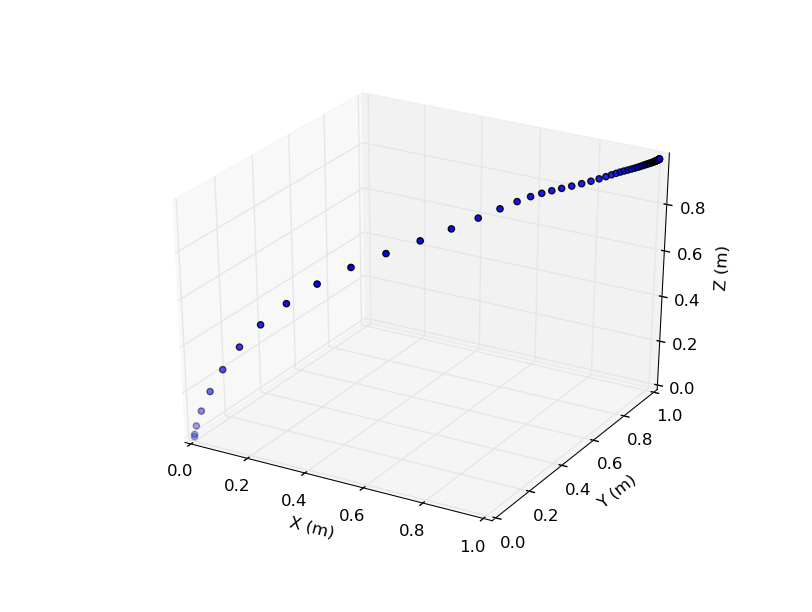
\includegraphics[width=\textwidth]{Figures/typical_run_time_3D_path.png}
		\rule{35em}{0.5pt}
	\caption[Typical Run 3D Path]{A typical run - the 3D path}
	\label{fig:Typical Run 3D Path}
\end{figure}

\begin{figure}[htbp]
	\centering
		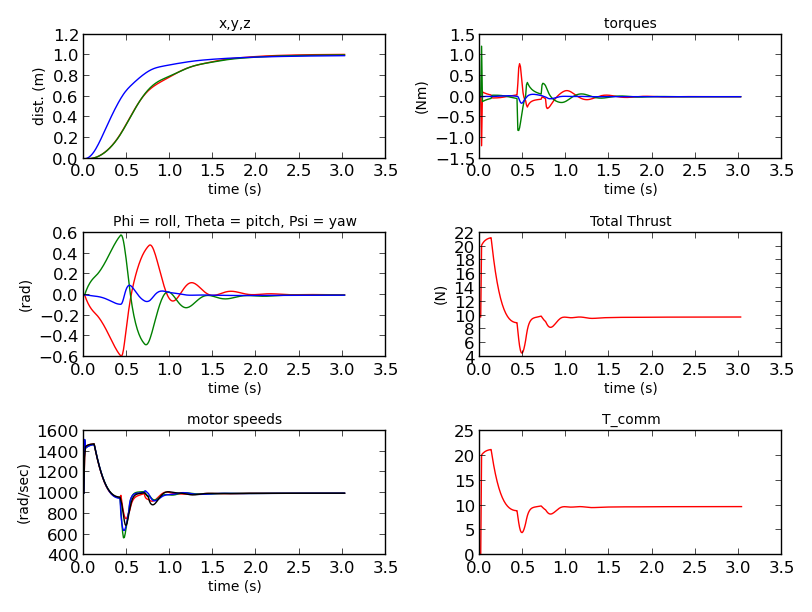
\includegraphics[width=\textwidth]{Figures/typical_run_time_domain.png}
		\rule{35em}{0.5pt}
	\caption[Typical Run Time Domain]{A typical run - time domain}
	\label{fig:Typical Run Time Domain}
\end{figure}


\begin{table}
\label{table:params}
\begin{doublespace}
\centering
\begin{tabular}{l l l}
    Simulation\\ Parameters & Units & Description\\
    \hline
    $g = -9.81            $& $ \frac{m}{s^2}          $ & acceleration due to gravity\\
    $m = 1                $& $ kg                      $ & mass\\
    $L = 1                $& $ m                       $ & length of quad-rotor arm\\
    $b = 10^{-6}          $& $ \frac{N m s^2}{Rad^2}  $ & aerodynamic torque coefficient\\
    $k = 2.45*10^{-6}     $& $ \frac{N s^2}{Rad^2}    $ & aerodynamic thrust coefficient\\
    $Ixx = 5.0*10^{-3}    $& $ \frac{N m s^2}{Rad}    $ & moments of inertia \\
    $Iyy = 5.0*10^{-3}    $& $ \frac{N m s^2}{Rad}    $ & \\
    $Izz = 10.0*10^{-3}   $& $ \frac{N m s^2}{Rad}    $ & \\
    \hline
\end{tabular}
\caption[Simulation Parameters]{Simulation Parameters}
\end{doublespace}
\end{table}

\begin{figure}[htbp]
	\centering
		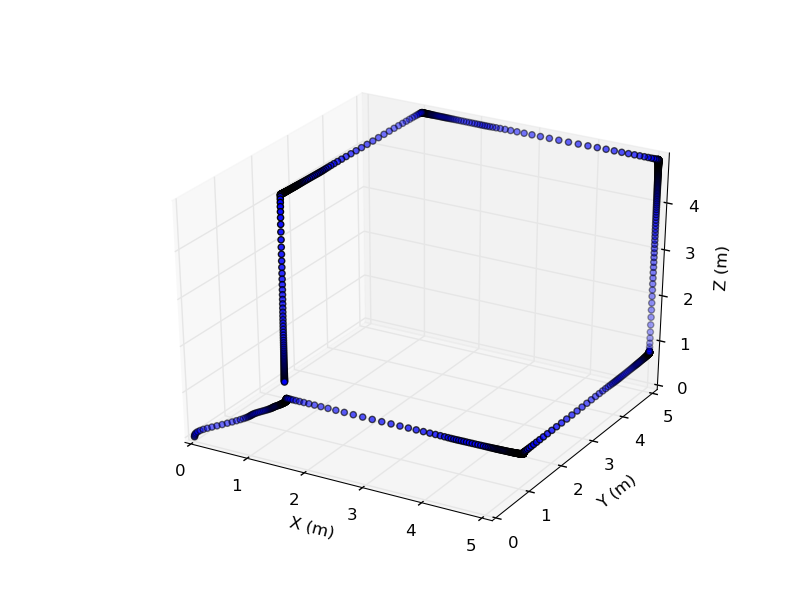
\includegraphics[width=\textwidth]{Figures/CubeEdges3D.png}
		\rule{35em}{0.5pt}
	\caption[Cube Edges 3D]{Tracing some of the edges of a 4m cube - the 3D path}
	\label{fig:Cube Edges 3D}
\end{figure}

\begin{figure}[htbp]
	\centering
		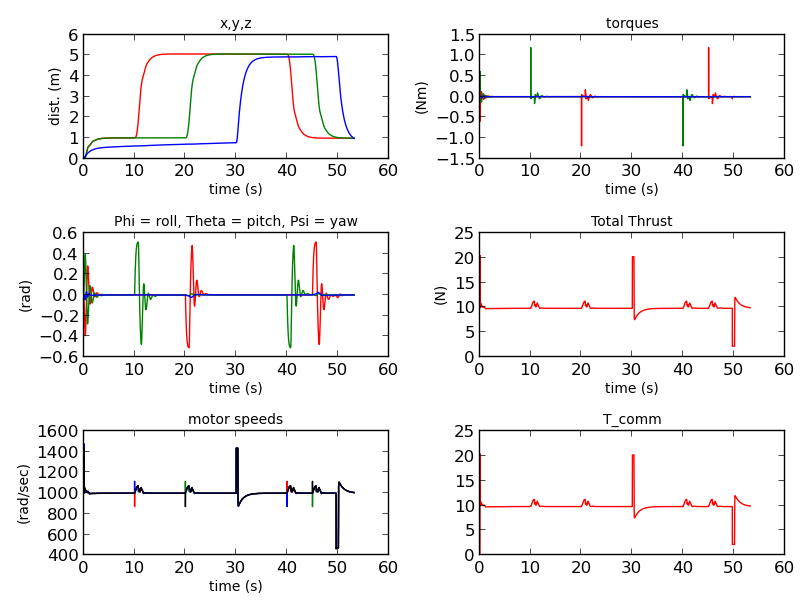
\includegraphics[width=\textwidth]{Figures/CubeEdgesGraphs.png}
		\rule{35em}{0.5pt}
	\caption[Cube Edges Time Domain]{Tracing some of the edges of a 4m cube - time domain plots}
	\label{fig:Cube Edges Time Domain}
\end{figure}


\begin{figure}[htbp]
	\centering
		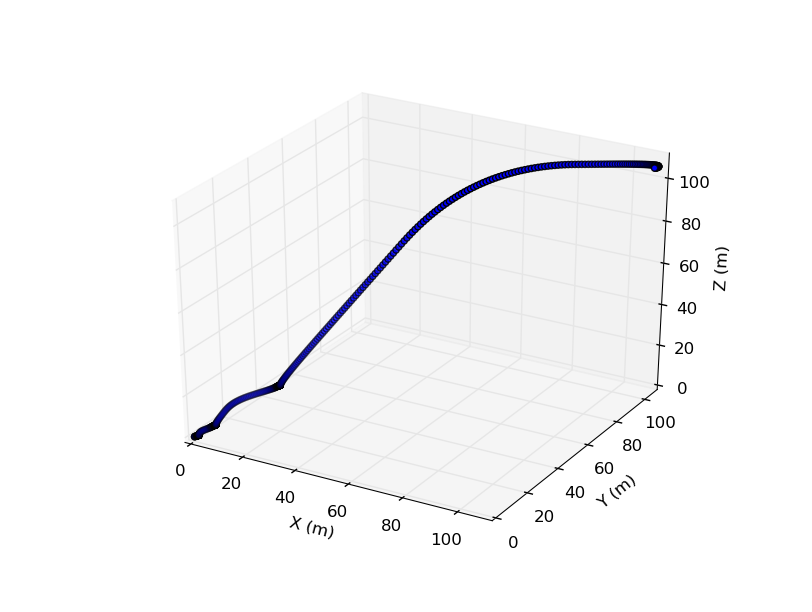
\includegraphics[width=\textwidth]{Figures/largeSetpointDifferencesTest_3d.png}
		\rule{35em}{0.5pt}
	\caption[Large Set Points 3D Path]{Testing the control with larger set points - the 3D path}
	\label{fig:Large Setpoints 3D Path}
\end{figure}

\begin{figure}[htbp]
	\centering
		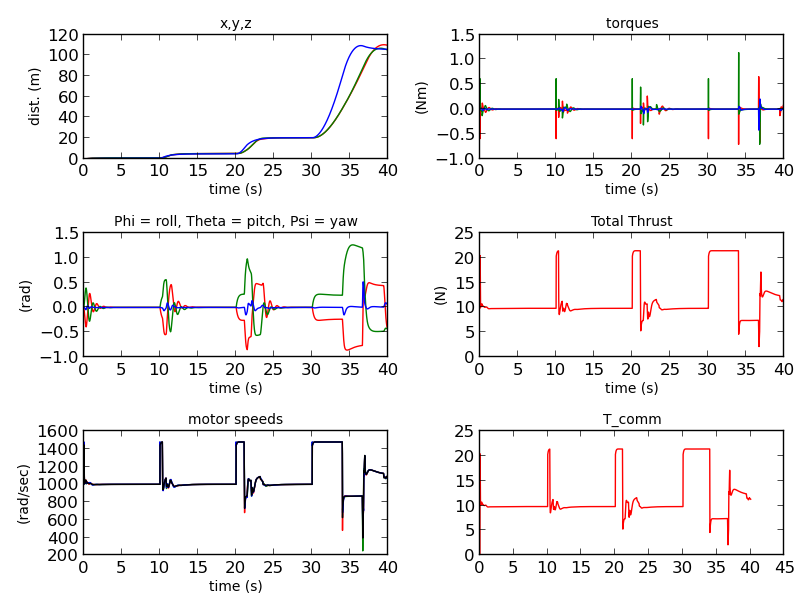
\includegraphics[width=\textwidth]{Figures/largeSetpointDifferencesTest_timedomain.png}
		\rule{35em}{0.5pt}
	\caption[Large Set Point Time Domain]{Testing the control with larger set points - time domain plots }
	\label{fig:Large Setpoint Time Domain}
\end{figure}





 
% Chapter Template

\chapter{PID Gain Optimization} % Main chapter title

\label{Chapter7} % Change X to a consecutive number; for referencing this chapter elsewhere, use \ref{ChapterX}

\lhead{Chapter 7. \emph{PID Gain Optimization}} % Change X to a consecutive number; this is for the header on each page - perhaps a shortened title

%----------------------------------------------------------------------------------------

In order to arrive at a solution to the quad-rotor energy optimization problem that is closer to running in real-time, a heuristic approach has been adopted. Recall that our general aim is to effectively control the vector position of the quad-rotor and additionally use the least energy in doing so. The relative simplicity of a PID controller makes it a good choice instead of the full nonlinear classical optimal control formulation. Also, if the PID control expressions are tuned well and that tuning is not changed, the control algorithm performs well. 

The motivation for our heuristic method is to find the PID controller tuning which uses the least energy to drive the UAV to the desired state. The PID tuning defines the dynamics of the controller. Using the quad-rotor model derived in chapter 3, the performance of the controller and the dynamics of the system can be evaluated as a function of the tuning. Mathematically, this can be represented as follows. 

The aim of the optimization is to find: $ argmin \big[  \sum_{k,i} \omega_i[k] \text{ } | \text{ } K_p , K_i , K_d  \big]  $ , where $\omega_i[k]$ is the $ith$ rotor speed at the $kth$ time step. The variables $K_p$ , $K_i$ and $K_d$ are the vectors of proportional, integral, and derivative gains defined as:

\begin{center}
$ K_p = \left[ \begin{array}{c} k_{px} \\ k_{py} \\ k_{pz}  \end{array} \right] , K_i = \left[ \begin{array}{c} k_{ix} \\ k_{iy} \\ k_{iz}  \end{array} \right], K_d = \left[ \begin{array}{c} k_{dx} \\ k_{dy} \\ k_{dz}  \end{array} \right] $  
\end{center}

In our simulations, the time integral of all four motor speeds is proportional to the total energy used. Calculation of the actual energy used by the UAV in traversing a flight path would require a model for the motor. This is seen as unnecessary for our purposes since the time integral of the motor speeds and the total energy used will have the same effective minimum. Since the control input is calculated as part of the control algorithm anyway, it is used as a performance metric.


In any realistic application of UAV technology, the energy budget is only one important aspect of the control problem. Other important criteria for evaluating the performance of a controller are over-shoot of the desired location, the time of flight, and mathematical resonances or marginal instabilities. These factors must be considered in the design of the system. However, in the initial results described below, the time integral of the motor speeds is used as a single performance metric. The reason for this is to simplify the relationship between the performance metric and the PID gains. This is described in the next section.


\section{Initial Simulation Results}

In the context of the optimization process described in the previous section, there is evidence for the lack of robustness of the PID control. This can be shown by analyzing the relationship between the measured total thrust and the PID gains. Ideally, a gradient descent method would be used to minimize the thrust as a function of the control gains. The basic flow of the algorithm that we would really like to implement is as follows.

\begin{itemize}
\item choose a set of proportional and derivative gains for each vector direction (x,y, and,z),
\item perform a simulation that controls the quad-rotor from an initial vector position to a desired vector position  
\item calculate the sum of the four motor speeds over the duration of the simulation
\item appropriately change the PID gains such that the sum of the motor speeds decreases
\item repeat until the sum of the motor speeds is found to be a minimum.
\end{itemize}

In reality, is has been found that the relationship between the measured total thrust and PID gains is not well behaved. After many days of trying to debug a gradient descent algorithm, and observing inconsistent behavior, it was decided that a brute force method might be the only possibility. A deeper understanding of the objective function was needed. The brute force method simply requires that we simulate the system and determine the value of the performance criteria for each possible set of PID gain vectors within a given range. 

In order limit the number of simulations required to really represent the dynamics of the system, the set point $(0,0,1)$ was chosen. By choosing this set point, the motion of the quad-rotor is intentionally limited to the z-direction which limits the number of possible gain vectors for this test. This makes the tuning of the $x$ and $y$ direction controllers irrelevant. To further limit the number of simulations required, the Ziegler-Nichols PID tuning method was used. This method is discussed in \cite{ziegler1942optimum}. Also, there is a wonderful Wikipedia page: \url{http://en.wikipedia.org/wiki/Ziegler-Nichols_method} . 

The Ziegler-Nichols method specifies simple algebraic relationships between the proportional, integral, and derivative gains. This allows each of the PID gains to be expressed as a function of a single gain variable, $k_u$ , which is allowed to range from 1 to 100.




 The results of these simulations are shown in Figure \ref{fig:ku vs thrust}.

 
\begin{figure}[htbp]
	\centering
		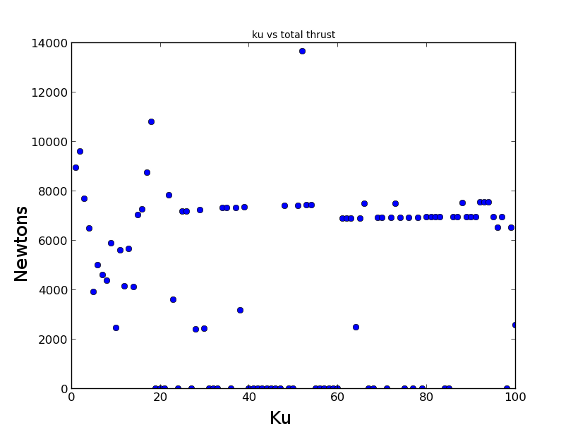
\includegraphics{Figures/kuvsthrust.png}
		\rule{35em}{0.5pt}
	\caption[ku vs thrust]{The relationship between Ku and the measured total thrust.}
	\label{fig:ku vs thrust}
\end{figure}

The relationship between Ku and the total measured thrust depicted in Figure \ref{fig:ku vs thrust} is rather disappointing to say the least. The values of zero total thrust are the result of simulations that failed to converge to the set point. Without an objective function that is at least marginally well behaved we have no hope to employ a gradient descent minimization technique. The relationship shown in Figure \ref{fig:ku vs thrust} is indeed a product of a deterministic system but displays little to no continuity. There are a few outliers in the data which are substantially lower in measured total thrust but the reason for their presence in the data as outliers is glib. 

Another detail which cannot be ignored is that the total thrust alone is not sufficient as a performance criteria. Additionally, for appropriate control of the UAV,  the overshoot and oscillations which show up in improperly tuned PID controllers must be accounted for. Specifically, as the proportional gain is increased to drive the system to the desired location more quickly, the total thrust for the simulation will decrease but eventually the overshoot and oscillations grow to unacceptable levels. In the opposite fashion, if the differential gain is increased, the overshoot and oscillations will be suppressed but the time required to reach the set point will increase along with the total thrust. The competitive nature of these three (necessary) performance criteria further complicate the relationship between the PID gain vectors and the objective function making a gradient descent minimization technique even less viable. 

 
\section{Brute Force Simulation Results}

Given that a standard mathematical optimization technique is out of the question, what options are left? With another year of research, a nonlinear control law could be implemented and would perhaps make the optimization possible, but this is uncertain. Sadly a naive, brute force approach is actually \textit{MORE} time efficient when compared to another year of research! For the sake of learning, a brute force algorithm is not so valuable. However, another year of research is simply not an option.

The decision was thus made to simply try many (many) possible gain vectors and have an appropriate objective function to characterize each of the simulations. Given that  the brute force algorithm is easy to write (and massively parallel-izable), around 6000 simulations were performed over a period of several hours. The computation was delegated two six independent instantiations of a python script, each one taking on a subset of the possible gain vectors and a separate CPU. 

A separate script was used to parse through all the results of the simulations which were stored in many time-stamped files. Of the roughly 6000 simulations, about 1000 of them ran to completion without a numerical explosion. For these, the set point was reached and the stopping criteria for the simulation were satisfied. Of the 1000 or so good runs, about 80 simulations satisfied the maximum overshoot and oscillation criteria. Only the gain vectors which produced less than ten percent overshoot were accepted. Likewise, only simulations which crossed the desired set point in each direction fewer than four times were deemed acceptable. The remaining 80 simulations were sorted lowest to highest by total measured thrust. The optimal run that was found is detailed in Table \ref{table:optimalrun} .   


\begin{table}\label{table:optimalrun}
\begin{doublespace}
\centering
\begin{tabular}{l l}
The Optimal Run      \\
\hline                        
kpx                 & 15 \\
kpy                 & 15 \\
kpz                 & 40 \\
kix                 & 0.8 \\
kiy                 & 0.8 \\
kiz                 & 15 \\
kdx                 & 10 \\
kdy                 & 10 \\
kdz                 & 50 \\
ending iteration    & 987 \\
discrete time step   & 0.01 (s)\\
flight time         & 9.87 (s) \\
cpu runtime         & 11.41 (s)\\
return value        & 1 (great success)\\
initial position    & [0, 0, 1] (m)\\
set point           & [1, 1, 2] (m) \\
total thrust        & 4969.8 (Newton seconds) \\
x crossings         & 3 \\
x overshoot         & 0.0249 (m) \\
y crossings         & 1 \\
y overshoot         & 0.0185 (m)\\
z crossings         & 1 \\
z overshoot         & 0.0992 (m) \\
\end{tabular}
\end{doublespace}
\end{table}

{\color{red} THE TABLE GOES HERE... }

In Figures \ref{fig:optimal run 3D path} and \ref{fig:optimal run time domain} the dynamics of the system with optimal PID tuning are shown. 

\begin{figure}[htbp]
	\centering
		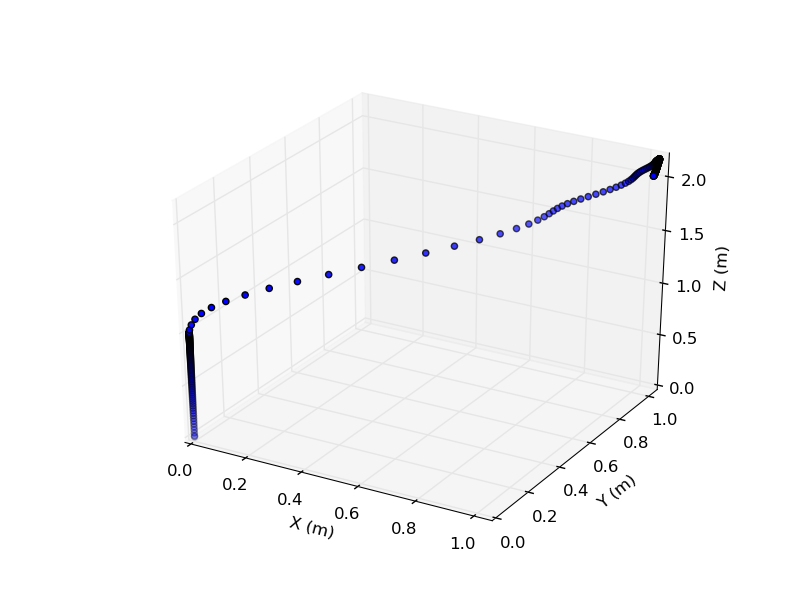
\includegraphics[width=\textwidth]{Figures/optimal_run_3D_path.png}
		\rule{35em}{0.5pt}
	\caption[optimal run 3D path]{The Optimal Run - 3D path}
	\label{fig:optimal run 3D path}
\end{figure}


\begin{figure}[htbp]
	\centering
		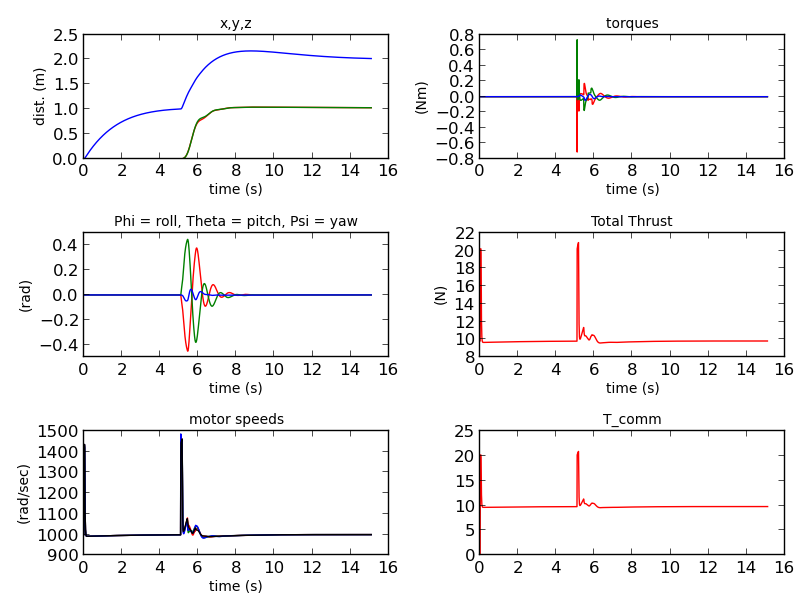
\includegraphics[width=\textwidth]{Figures/optimal_run_time_domain.png}
		\rule{35em}{0.5pt}
	\caption[optimal run time domain]{The Optimal Run - time domain}
	\label{fig:optimal run time domain}
\end{figure}


{\color{red} THE FIGURES GO HERE... }

Figures \ref{fig:optimal run 3D path} and \ref{fig:optimal run time domain} show the simulation of the quad-rotor flight from the initial point $(0,0,1)$ to the desired point $(1,1,2)$ using the optimal PID tuning. There are actually two distinct legs to the simulation. The reason for this comes from the fact that there are two types of initial conditions which have fundamental differences. There is a hovering state which we use as initial conditions for the simulations in the optimization procedure. There is another mathematical state which occurs at the very beginning of the simulation. The mathematical initialization of the quad-rotor state is at the origin $(0,0,0)$ with zero velocity and acceleration but it is not exactly hovering. This subtle distinction comes from the fact that the force of gravity is not canceled out by the thrust initially. The controller has had no time to act to stabilize the system. The physical scenario that this condition would correspond to is if a person held the quad-rotor at the initial position in free space (perhaps designated as the origin) and then at $t=0$, simply let go. Another way to state this is that the simulations do not account for the normal force which would be imparted to the quad-rotor if it were simply taking off from the ground. To account for this would perhaps require augmentation of the dynamical model of the quad-rotor. 

It is our aim was to start and end in a hovering state for the optimization. This is why our simulations start with a 'take-off sequence' where the quad-rotor leaves from the origin and goes to the position $(0,0,1)$. After this, the system is stabilized in a hovering state. From there, arbitrary paths can be incrementally constructed by simply redefining the desired location.

Despite the mathematical difficulties that were experienced with the various optimization techniques that were explored, this final result is useful. Until a reasonable mathematical optimization technique is found, the optimality of the solution described above is a function of how much time one is willing to run the brute force algorithm. 
































% Chapter Template

\chapter{Summary and Future Work} % Main chapter title

\label{Chapter8}

\lhead{Chapter 8. \emph{Conclusion}}

\section{Summary}
In this final chapter we review the main points of the paper and propose directions for further work. Our first significant result was the dynamic model of the quad-rotor. The Euler-Lagrange formulation was used to derive the dynamic model. The resulting set of nonlinear differential equations formed the basis for both the control and optimization methods which were subsequently derived.

Our first approach to the path-energy optimization problem which incorporated the dynamic model was classical optimal control. Using this formulation, we derived a set of differential and algebraic equations which form a complex boundary value problem. Our initial aim was to develop a method for achieving a path-energy optimization which would perform on a near-real-time-schedule. The computational resources needed to solve the optimal control boundary value problem on this real-time schedule invalidate it as a possible solution.

The next method of optimization which was explored was a heuristic method. Control of the UAV was attained by way of a set of PID and PD controllers. Since the performance of the quad-rotor is defined by the controller tuning, the system can be optimized as a function of this tuning. Relevant criteria for evaluating the performance of the system are the total thrust integrated over the duration of the simulation, oscillations that the system experiences, overshoot of the desired location, and the total time of flight. It was determined experimentally that the relationship between these performance metrics and the controller tuning was not well-behaved mathematically. Without a clean mathematical representation of our objective function, the viability of an efficient optimization method is questioned.

Next, a brute force method was used to determine the optimal controller tuning. With limited time, the true optimality of the solution is not certain. Even with limited resources we were able to determine a controller tuning which is good enough to perform simulated fights in a relatively efficient manner.

\section{Further Work}

The problem of path-energy optimization as solved in this thesis can be worked on in the future to produce more robust results. Two possible mathematical modifications that could possibly allow for an efficient optimization algorithm are as follows. They both have design trade-offs.

\begin{itemize}

\item \textit{Model Linearization} One approach would beto use a linearized model. The goal there would be to simplify the relationship between the controller tuning and the relevant performance metrics by simplifying the mathematical representation of the dynamic model. The danger in using a linear approximation is creating an over-simplified model that is divergent from reality to an extent that makes it unusable.

\item \textit{Nonlinear Control}If instead of a linear PID controller, a nonlinear control method was used, the stability of the system could be increased. This would perhaps allow for a well behaved and more well defined relationship between the parameters of the controller and the measurable dynamics of the system. The obvious caveat  here is the increase in complexity of the controller. The only real way to know if one of these options would allow for an efficient optimization procedure would be to try them all and characterize them in the context of the goal of the flight.

\item \textit{UAV Swarm Optimization} Another area of research interest that would benefit from an energy optimization procedure is the control of swarms of UAVs. The distributed control of UAVs is a field which offers a wide range of engineering challenges such as collision avoidance, optimization of networked communication, and optimization of workload delegation toward a common goal. The contextual details of the cooperative aim of the swarm would inform the optimization of the system.


\item \textit{Sensor Fusion and State Estimation} Yet another area of possible further research is in the sensor fusion and state estimation problem. For a physical implementation, knowledge of the state of the system is a critical component. Given that there are a very large variety of physical sensors that could contribute to this knowledge, this is an interesting problem. An aspect of this problem that adds richness to this situation is the fact that each type of sensor will have a different rate at which physical information is available. This rate is determined by the physical nature of the quantity being measured. A good example is the integration of GPS measurements and accelerometer measurements. Values from these sensors are available perhaps at rates of 1 Hz and 100 Hz respectively. The sensor data would be integrated with a Kalman filter to develop situational awareness which allows for effective control of the system.
\end{itemize}

In general the control and optimization of UAVs is a rich and evolving field of research with many unsolved problems. There will be many commercial applications of this technology appearing in coming years which will be informed by future research.













%\input{Chapters/Chapter5} 
%\input{Chapters/Chapter6} 
%\input{Chapters/Chapter7} 

%----------------------------------------------------------------------------------------
%	THESIS CONTENT - APPENDICES
%----------------------------------------------------------------------------------------

\addtocontents{toc}{\vspace{2em}} % Add a gap in the Contents, for aesthetics

\appendix % Cue to tell LaTeX that the following 'chapters' are Appendices

% Include the appendices of the thesis as separate files from the Appendices folder
% Uncomment the lines as you write the Appendices

% Appendix A

\chapter{Dynamic system model and PID control - agentModule.py} % Main appendix title

\label{AppendixA} % For referencing this appendix elsewhere, use \ref{AppendixA}

% This is for the header on each page - perhaps a shortened title
\lhead{Appendix A. \emph{agentModule.py}}



\lstinputlisting[language=Python]{/home/ek/Dropbox/THESIS/python_scripts/agent_module.py}




 % agent module
% Appendix b

\chapter{A module for updating the PID set point - waypointNavigation.py} % Main appendix title

\label{AppendixB} % For referencing this appendix elsewhere, use \ref{AppendixA}

% This is for the header on each page - perhaps a shortened title
\lhead{Appendix B. \emph{waypointNavigation.py}}



\lstinputlisting[language=Python]{/home/ek/Dropbox/THESIS/python_scripts/waypoint_navigation.py}




 % waypoint navigation
% Appendix C

\chapter{Functions used in the brute force method - bruteForceFunctions.py} % Main appendix title

\label{AppendixC} % For referencing this appendix elsewhere, use \ref{AppendixA}

% This is for the header on each page - perhaps a shortened title
\lhead{Appendix C. \emph{bruteForceFunctions.py}}



\lstinputlisting[language=Python]{/home/ek/Dropbox/THESIS/python_scripts/brute_force_functions.py}




 % brute force functions
% Appendix D

\chapter{runSimsBruteForce.py} % Main appendix title

\label{AppendixD} % For referencing this appendix elsewhere, use \ref{AppendixA}

% This is for the header on each page - perhaps a shortened title
\lhead{Appendix D. \emph{runSimsBruteForce.py}} 



\lstinputlisting[language=Python]{/home/ek/Dropbox/THESIS/python_scripts/run_sims_brute_force.py}




 % run sims brute force
% Appendix E

\chapter{A module to sort the results of the brute force method - parseResults.py} % Main appendix title

\label{AppendixE} % For referencing this appendix elsewhere, use \ref{AppendixA}

% This is for the header on each page - perhaps a shortened title
\lhead{Appendix E. \emph{parseResults.py}}



\lstinputlisting[language=Python]{/home/ek/Dropbox/THESIS/python_scripts/parse_results.py}




 % parse_results
% Appendix F

\chapter{Finite difference method applied to the optimal control BVP -  finiteDiffSolution.py} % Main appendix title

\label{AppendixF} % For referencing this appendix elsewhere, use \ref{AppendixA}

% This is for the header on each page - perhaps a shortened title
\lhead{Appendix F. \emph{finiteDiffSolution.py}}



\lstinputlisting[language=Python]{/home/ek/Dropbox/THESIS/quadrotor_optimal_control/finiteDiffSolution.py}




 % finite diff solution



\addtocontents{toc}{\vspace{2em}} % Add a gap in the Contents, for aesthetics

\backmatter

%----------------------------------------------------------------------------------------
%	BIBLIOGRAPHY
%----------------------------------------------------------------------------------------

\label{Bibliography}

\lhead{\emph{Bibliography}} % Change the page header to say "Bibliography"

\bibliographystyle{unsrtnat} % Use the "unsrtnat" BibTeX style for formatting the Bibliography

\bibliography{Bibliography}%,IEEEexample,IEEEabrv} % The references (bibliography) information are stored in the file named "Bibliography.bib"

\end{document}  
